% Options for packages loaded elsewhere
% Options for packages loaded elsewhere
\PassOptionsToPackage{unicode}{hyperref}
\PassOptionsToPackage{hyphens}{url}
\PassOptionsToPackage{dvipsnames,svgnames,x11names}{xcolor}
%
\documentclass[
  letterpaper,
  DIV=11,
  numbers=noendperiod]{scrreprt}
\usepackage{xcolor}
\usepackage{amsmath,amssymb}
\setcounter{secnumdepth}{2}
\usepackage{iftex}
\ifPDFTeX
  \usepackage[T1]{fontenc}
  \usepackage[utf8]{inputenc}
  \usepackage{textcomp} % provide euro and other symbols
\else % if luatex or xetex
  \usepackage{unicode-math} % this also loads fontspec
  \defaultfontfeatures{Scale=MatchLowercase}
  \defaultfontfeatures[\rmfamily]{Ligatures=TeX,Scale=1}
\fi
\usepackage{lmodern}
\ifPDFTeX\else
  % xetex/luatex font selection
  \setmainfont[]{Arimo}
  \setsansfont[]{Poppins}
\fi
% Use upquote if available, for straight quotes in verbatim environments
\IfFileExists{upquote.sty}{\usepackage{upquote}}{}
\IfFileExists{microtype.sty}{% use microtype if available
  \usepackage[]{microtype}
  \UseMicrotypeSet[protrusion]{basicmath} % disable protrusion for tt fonts
}{}
\makeatletter
\@ifundefined{KOMAClassName}{% if non-KOMA class
  \IfFileExists{parskip.sty}{%
    \usepackage{parskip}
  }{% else
    \setlength{\parindent}{0pt}
    \setlength{\parskip}{6pt plus 2pt minus 1pt}}
}{% if KOMA class
  \KOMAoptions{parskip=half}}
\makeatother
% Make \paragraph and \subparagraph free-standing
\makeatletter
\ifx\paragraph\undefined\else
  \let\oldparagraph\paragraph
  \renewcommand{\paragraph}{
    \@ifstar
      \xxxParagraphStar
      \xxxParagraphNoStar
  }
  \newcommand{\xxxParagraphStar}[1]{\oldparagraph*{#1}\mbox{}}
  \newcommand{\xxxParagraphNoStar}[1]{\oldparagraph{#1}\mbox{}}
\fi
\ifx\subparagraph\undefined\else
  \let\oldsubparagraph\subparagraph
  \renewcommand{\subparagraph}{
    \@ifstar
      \xxxSubParagraphStar
      \xxxSubParagraphNoStar
  }
  \newcommand{\xxxSubParagraphStar}[1]{\oldsubparagraph*{#1}\mbox{}}
  \newcommand{\xxxSubParagraphNoStar}[1]{\oldsubparagraph{#1}\mbox{}}
\fi
\makeatother

\usepackage{color}
\usepackage{fancyvrb}
\newcommand{\VerbBar}{|}
\newcommand{\VERB}{\Verb[commandchars=\\\{\}]}
\DefineVerbatimEnvironment{Highlighting}{Verbatim}{commandchars=\\\{\}}
% Add ',fontsize=\small' for more characters per line
\usepackage{framed}
\definecolor{shadecolor}{RGB}{241,243,245}
\newenvironment{Shaded}{\begin{snugshade}}{\end{snugshade}}
\newcommand{\AlertTok}[1]{\textcolor[rgb]{0.68,0.00,0.00}{#1}}
\newcommand{\AnnotationTok}[1]{\textcolor[rgb]{0.37,0.37,0.37}{#1}}
\newcommand{\AttributeTok}[1]{\textcolor[rgb]{0.40,0.45,0.13}{#1}}
\newcommand{\BaseNTok}[1]{\textcolor[rgb]{0.68,0.00,0.00}{#1}}
\newcommand{\BuiltInTok}[1]{\textcolor[rgb]{0.00,0.23,0.31}{#1}}
\newcommand{\CharTok}[1]{\textcolor[rgb]{0.13,0.47,0.30}{#1}}
\newcommand{\CommentTok}[1]{\textcolor[rgb]{0.37,0.37,0.37}{#1}}
\newcommand{\CommentVarTok}[1]{\textcolor[rgb]{0.37,0.37,0.37}{\textit{#1}}}
\newcommand{\ConstantTok}[1]{\textcolor[rgb]{0.56,0.35,0.01}{#1}}
\newcommand{\ControlFlowTok}[1]{\textcolor[rgb]{0.00,0.23,0.31}{\textbf{#1}}}
\newcommand{\DataTypeTok}[1]{\textcolor[rgb]{0.68,0.00,0.00}{#1}}
\newcommand{\DecValTok}[1]{\textcolor[rgb]{0.68,0.00,0.00}{#1}}
\newcommand{\DocumentationTok}[1]{\textcolor[rgb]{0.37,0.37,0.37}{\textit{#1}}}
\newcommand{\ErrorTok}[1]{\textcolor[rgb]{0.68,0.00,0.00}{#1}}
\newcommand{\ExtensionTok}[1]{\textcolor[rgb]{0.00,0.23,0.31}{#1}}
\newcommand{\FloatTok}[1]{\textcolor[rgb]{0.68,0.00,0.00}{#1}}
\newcommand{\FunctionTok}[1]{\textcolor[rgb]{0.28,0.35,0.67}{#1}}
\newcommand{\ImportTok}[1]{\textcolor[rgb]{0.00,0.46,0.62}{#1}}
\newcommand{\InformationTok}[1]{\textcolor[rgb]{0.37,0.37,0.37}{#1}}
\newcommand{\KeywordTok}[1]{\textcolor[rgb]{0.00,0.23,0.31}{\textbf{#1}}}
\newcommand{\NormalTok}[1]{\textcolor[rgb]{0.00,0.23,0.31}{#1}}
\newcommand{\OperatorTok}[1]{\textcolor[rgb]{0.37,0.37,0.37}{#1}}
\newcommand{\OtherTok}[1]{\textcolor[rgb]{0.00,0.23,0.31}{#1}}
\newcommand{\PreprocessorTok}[1]{\textcolor[rgb]{0.68,0.00,0.00}{#1}}
\newcommand{\RegionMarkerTok}[1]{\textcolor[rgb]{0.00,0.23,0.31}{#1}}
\newcommand{\SpecialCharTok}[1]{\textcolor[rgb]{0.37,0.37,0.37}{#1}}
\newcommand{\SpecialStringTok}[1]{\textcolor[rgb]{0.13,0.47,0.30}{#1}}
\newcommand{\StringTok}[1]{\textcolor[rgb]{0.13,0.47,0.30}{#1}}
\newcommand{\VariableTok}[1]{\textcolor[rgb]{0.07,0.07,0.07}{#1}}
\newcommand{\VerbatimStringTok}[1]{\textcolor[rgb]{0.13,0.47,0.30}{#1}}
\newcommand{\WarningTok}[1]{\textcolor[rgb]{0.37,0.37,0.37}{\textit{#1}}}

\usepackage{longtable,booktabs,array}
\newcounter{none} % for unnumbered tables
\usepackage{calc} % for calculating minipage widths
% Correct order of tables after \paragraph or \subparagraph
\usepackage{etoolbox}
\makeatletter
\patchcmd\longtable{\par}{\if@noskipsec\mbox{}\fi\par}{}{}
\makeatother
% Allow footnotes in longtable head/foot
\IfFileExists{footnotehyper.sty}{\usepackage{footnotehyper}}{\usepackage{footnote}}
\makesavenoteenv{longtable}
\usepackage{graphicx}
\makeatletter
\newsavebox\pandoc@box
\newcommand*\pandocbounded[1]{% scales image to fit in text height/width
  \sbox\pandoc@box{#1}%
  \Gscale@div\@tempa{\textheight}{\dimexpr\ht\pandoc@box+\dp\pandoc@box\relax}%
  \Gscale@div\@tempb{\linewidth}{\wd\pandoc@box}%
  \ifdim\@tempb\p@<\@tempa\p@\let\@tempa\@tempb\fi% select the smaller of both
  \ifdim\@tempa\p@<\p@\scalebox{\@tempa}{\usebox\pandoc@box}%
  \else\usebox{\pandoc@box}%
  \fi%
}
% Set default figure placement to htbp
\def\fps@figure{htbp}
\makeatother

\ifLuaTeX
  \usepackage{luacolor}
  \usepackage[soul]{lua-ul}
\else
  \usepackage{soul}
\fi




\setlength{\emergencystretch}{3em} % prevent overfull lines

\providecommand{\tightlist}{%
  \setlength{\itemsep}{0pt}\setlength{\parskip}{0pt}}



 


\usepackage{fontspec}
\usepackage{multirow}
\usepackage{multicol}
\usepackage{colortbl}
\usepackage{ulem}
\usepackage{hhline}
\newlength\Oldarrayrulewidth
\newlength\Oldtabcolsep
\usepackage{longtable}
\usepackage{array}
\usepackage{hyperref}
\usepackage{float}
\usepackage{wrapfig}
\usepackage{booktabs}
\usepackage{array}
\usepackage{graphicx}
\usepackage{xcolor}
\usepackage{eso-pic}

\renewcommand{\arraystretch}{1.2}

\AtBeginDocument{\let\maketitle\relax}
\usepackage{float}
\KOMAoption{captions}{tableheading}
\makeatletter
\@ifpackageloaded{tcolorbox}{}{\usepackage[skins,breakable]{tcolorbox}}
\@ifpackageloaded{fontawesome5}{}{\usepackage{fontawesome5}}
\definecolor{quarto-callout-color}{HTML}{909090}
\definecolor{quarto-callout-note-color}{HTML}{0758E5}
\definecolor{quarto-callout-important-color}{HTML}{CC1914}
\definecolor{quarto-callout-warning-color}{HTML}{EB9113}
\definecolor{quarto-callout-tip-color}{HTML}{00A047}
\definecolor{quarto-callout-caution-color}{HTML}{FC5300}
\definecolor{quarto-callout-color-frame}{HTML}{acacac}
\definecolor{quarto-callout-note-color-frame}{HTML}{4582ec}
\definecolor{quarto-callout-important-color-frame}{HTML}{d9534f}
\definecolor{quarto-callout-warning-color-frame}{HTML}{f0ad4e}
\definecolor{quarto-callout-tip-color-frame}{HTML}{02b875}
\definecolor{quarto-callout-caution-color-frame}{HTML}{fd7e14}
\makeatother
\makeatletter
\@ifpackageloaded{bookmark}{}{\usepackage{bookmark}}
\makeatother
\makeatletter
\@ifpackageloaded{caption}{}{\usepackage{caption}}
\AtBeginDocument{%
\ifdefined\contentsname
  \renewcommand*\contentsname{Table of contents}
\else
  \newcommand\contentsname{Table of contents}
\fi
\ifdefined\listfigurename
  \renewcommand*\listfigurename{List of Figures}
\else
  \newcommand\listfigurename{List of Figures}
\fi
\ifdefined\listtablename
  \renewcommand*\listtablename{List of Tables}
\else
  \newcommand\listtablename{List of Tables}
\fi
\ifdefined\figurename
  \renewcommand*\figurename{Figure}
\else
  \newcommand\figurename{Figure}
\fi
\ifdefined\tablename
  \renewcommand*\tablename{Table}
\else
  \newcommand\tablename{Table}
\fi
}
\@ifpackageloaded{float}{}{\usepackage{float}}
\floatstyle{ruled}
\@ifundefined{c@chapter}{\newfloat{codelisting}{h}{lop}}{\newfloat{codelisting}{h}{lop}[chapter]}
\floatname{codelisting}{Listing}
\newcommand*\listoflistings{\listof{codelisting}{List of Listings}}
\makeatother
\makeatletter
\makeatother
\makeatletter
\@ifpackageloaded{caption}{}{\usepackage{caption}}
\@ifpackageloaded{subcaption}{}{\usepackage{subcaption}}
\makeatother
\usepackage{bookmark}
\IfFileExists{xurl.sty}{\usepackage{xurl}}{} % add URL line breaks if available
\urlstyle{same}
\hypersetup{
  pdftitle={Developable Land Inventory},
  pdfauthor={CT Office of Policy and Management, GIS Office},
  colorlinks=true,
  linkcolor={blue},
  filecolor={Maroon},
  citecolor={Blue},
  urlcolor={Blue},
  pdfcreator={LaTeX via pandoc}}


\title{Developable Land Inventory}
\usepackage{etoolbox}
\makeatletter
\providecommand{\subtitle}[1]{% add subtitle to \maketitle
  \apptocmd{\@title}{\par {\large #1 \par}}{}{}
}
\makeatother
\subtitle{Technical Guidance}
\author{CT Office of Policy and Management, GIS Office}
\date{}
\begin{document}
\maketitle

\clearpage
\thispagestyle{empty}

\AddToShipoutPictureBG*{
  \includegraphics[
    width=\paperwidth,
    height=\paperheight,
    keepaspectratio=false
  ]{images/DLI_cover.png}
}

\null
\clearpage

\renewcommand*\contentsname{Table of contents}
{
\setcounter{tocdepth}{4}
\tableofcontents
}

\bookmarksetup{startatroot}

\chapter*{Summary}\label{summary}
\addcontentsline{toc}{chapter}{Summary}

\markboth{Summary}{Summary}

The \emph{Developable Land Inventory Technical Guidance}, prepared by
the Connecticut Office of Policy and Management's GIS Office, provides a
standardized, transparent framework for municipalities to identify a
``developable land inventory'', a preliminary screening level product,
as defined in
\href{https://cga.ct.gov/2026/sup/chap_124b.htm\#sec_8-13aa}{Connecticut
General Statutes (C.G.S.) Sec. 8-13aa}. This is required as part of the
Regional Housing Needs Assessment allocation requirements
(\href{https://cga.ct.gov/2026/sup/chap_124b.htm\#sec_8-13dd}{C.G.S.
Sec. 8-13dd}) and the municipal and regional Housing Growth Plans
(\href{https://cga.ct.gov/2026/sup/chap_124b.htm\#sec_8-13bb}{C.G.S.
Sec. 8-13bb and 8-13cc}), as well as a foundational piece of subsequent
suitability analyses as part of the a Housing Growth Plan. The guidance
outlines datasets, analytical methods, and mapping standards that can be
used to produce a consistent, statewide inventory of developable land.

The document emphasizes that identifying land as ``developable'' does
not obligate development, nor does exclusion from the inventory
permanently restrict future development opportunities. Instead, the
inventory serves as a foundational input to each municipality's Housing
Growth Plan, supporting other elements of the planning process. The
developable land inventory is not a permanent designation of a
property's development potential.

The developable land inventory is only one element of the broader
planning process required under these statutes. The diagram below shows
how it fits within that larger analysis.

\begin{center}
\pandocbounded{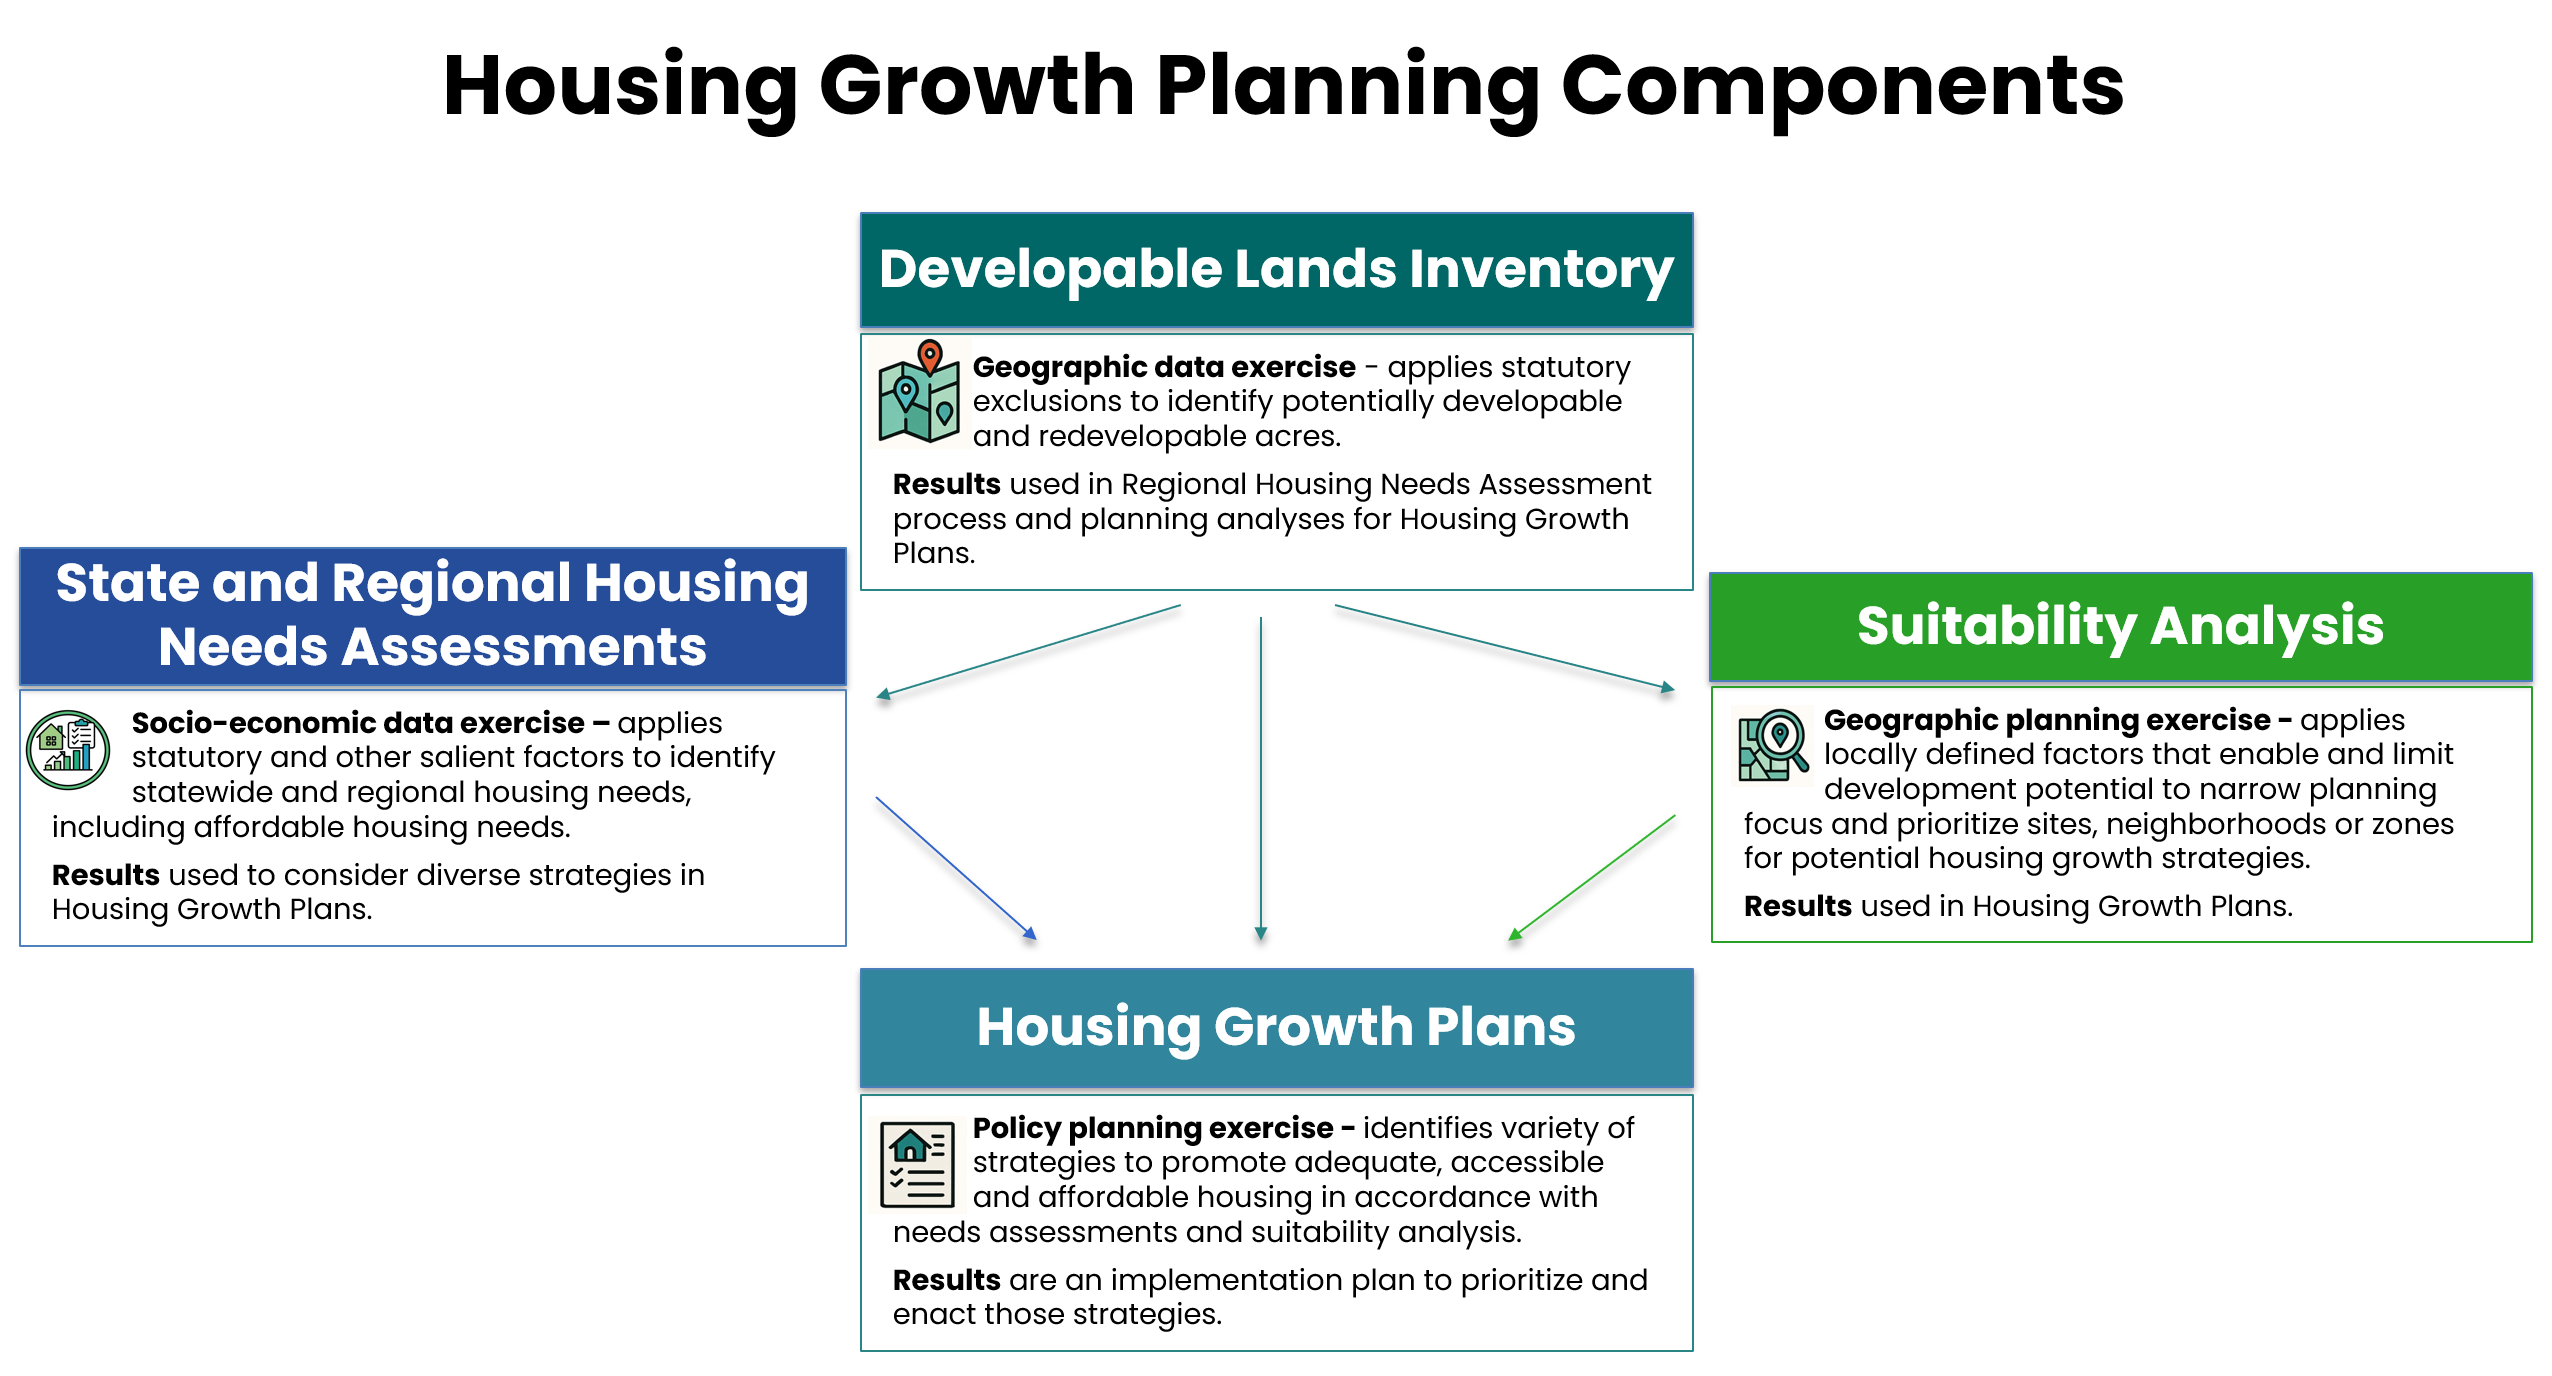
\includegraphics[keepaspectratio]{images/components.png}}
\end{center}

\section*{Use of This Analysis}\label{use-of-this-analysis}
\addcontentsline{toc}{section}{Use of This Analysis}

\markright{Use of This Analysis}

In the \textbf{Regional Housing Needs Assessment}, the following should
be included:

\begin{itemize}
\tightlist
\item
  A summary of developable land pursuant to Section 8-13aa for use in
  the Regional Housing Needs allocation.
\end{itemize}

In the subsequent \textbf{suitability analyses} of a Housing Growth
Plan:

\begin{itemize}
\tightlist
\item
  The developable land inventory serves as a foundation, with locally
  selected planning factors added to identify areas that could
  potentially enable or limit development.
\end{itemize}

As an element of a \textbf{Housing Growth Plan}, the following should be
included:

\begin{itemize}
\item
  Three town-wide maps showing statutory exclusions, developable land,
  vacant parcels, and potential redevelopment areas.
\item
  A narrative methodology describing data sources, queries, processing
  steps, and classification methods used in the analysis.
\end{itemize}

\section*{Statutory Definitions}\label{statutory-definitions}
\addcontentsline{toc}{section}{Statutory Definitions}

\markright{Statutory Definitions}

\href{https://cga.ct.gov/2026/sup/chap_124b.htm\#sec_8-13aa}{C.G.S. Sec.
8-13aa} defines what ``developable land'' is within the context of this
planning exercise. In addition to areas that are commercially feasible
for development, it outlines five categories of land that should be
excluded from the developable land inventory:

\begin{enumerate}
\def\labelenumi{\Alph{enumi}.}
\tightlist
\item
  Land already committed to public use or purpose (public or private)
\item
  Open space, parks, and recreation areas dedicated to the public or
  protected by a conservation easement
\item
  Land subject to enforceable restrictions or prohibitions on
  development
\item
  Wetlands or watercourses, as defined in the Wetlands and Watercourses
  Act (CGS Chapter 440)
\item
  Contiguous land areas of 0.5 acres or more that are unsuitable for
  development due to steep slopes or other topographic conditions
\end{enumerate}

For each category, the guidance identifies recommended datasets and
provides detailed instructions for filtering, querying, and validating
features.

\section*{Vacant and Redevelopable
Land}\label{vacant-and-redevelopable-land}
\addcontentsline{toc}{section}{Vacant and Redevelopable Land}

\markright{Vacant and Redevelopable Land}

Beyond statutory exclusions, municipalities are encouraged to identify:

\begin{itemize}
\item
  Vacant parcels
\item
  Potentially redevelopable parcels
\end{itemize}

These categories can help identify `commercially feasible'
opportunities, support later phases of the Housing Growth Plan process,
and inform future housing capacity assessments.

\section*{Mapping Standards}\label{mapping-standards}
\addcontentsline{toc}{section}{Mapping Standards}

\markright{Mapping Standards}

The guidance specifies three maps to be included in the Housing Growth
Plans:

\begin{enumerate}
\def\labelenumi{\arabic{enumi}.}
\item
  Statutory Exclusions Map
\item
  Developable Land Map
\item
  Developable Land Summary Map, including vacant and
  redevelopment-potential parcels
\end{enumerate}

\section*{Next Steps}\label{next-steps}
\addcontentsline{toc}{section}{Next Steps}

\markright{Next Steps}

The Developable Land Inventory is just one portion of the Housing Growth
Planning process. While this is a required element in the Housing Growth
Plans and the Regional Needs Assessments, separate analyses will apply
locally defined factors that enable and limit development potential to
narrow planning focus and prioritize site, neighborhoods, or zones for
potential housing growth strategies.

\bookmarksetup{startatroot}

\chapter{Introduction}\label{introduction}

\section{Purpose}\label{purpose}

This documentation provides technical guidance for preparing a municipal
developable land inventory required under
\href{https://cga.ct.gov/2026/sup/chap_124b.htm}{Connecticut General
Statutes (C.G.S.) Sec. 8-13aa -- 8-13dd}. The developable land inventory
is a preliminary, planning-level screening product for use in this
specific planning process, not a permanent or legal designation of
development potential.

This guidance serves as one of the statewide data tools that the CT GIS
Office within the Office of Policy and Management (OPM) is directed to
develop under statute, for use by municipalities and COGs, together with
local data, in compiling the developable land inventory.

\begin{quote}
\href{https://cga.ct.gov/2026/sup/chap_124b.htm\#sec_8-13dd}{C.G.S. Sec.
8-13dd(g)}: On or before July 1, 2026, and every five years thereafter,
the Geographic Information Systems Office within the Office of Policy
and Management, in consultation and coordination with the regional
councils of governments, shall develop \textbf{state-wide data tools for
municipalities to use, together with local data, to compile an inventory
of developable land}, as defined in section 8-13aa.
\end{quote}

The developable land inventory is used for two distinct statutory
purposes:

\begin{itemize}
\item
  \textbf{Regional Housing Needs Assessment allocations} (C.G.S. Sec.
  8-13dd), prepared exclusively by COGs

  and
\item
  \textbf{Housing Growth Plans} prepared by municipalities (C.G.S. Sec.
  8-13bb) or regional councils of governments (COGs) (C.G.S. Sec.
  8-13cc);
\end{itemize}

The inventory identifies land that meets the statutory definition of
developable land in
\href{https://cga.ct.gov/2026/sup/chap_124b.htm\#sec_8-13aa}{C.G.S. Sec.
8-13aa} and serves as a foundational input to both processes. This
guidance is intended to support a transparent analytical approach across
municipalities and COGs, while preserving flexibility in how each
community arrives at its final inventory.

\begin{tcolorbox}[enhanced jigsaw, arc=.35mm, bottomrule=.15mm, breakable, colback=white, colframe=quarto-callout-warning-color-frame, left=2mm, leftrule=.75mm, opacityback=0, rightrule=.15mm, toprule=.15mm]
\begin{minipage}[t]{5.5mm}
\textcolor{quarto-callout-warning-color}{\faExclamationTriangle}
\end{minipage}%
\begin{minipage}[t]{\textwidth - 5.5mm}

\vspace{-3mm}\textbf{A note about ``developable land''}\vspace{3mm}

Identifying land as developable does not obligate anyone to pursue
development on that land, nor does exclusion from the inventory limit
future development opportunities outside the context of the Housing
Growth Plan or Regional Needs Assessment process. The developable land
inventory is not a permanent designation of a property's development
potential. Rather, it is a necessary step in preparing a Housing Growth
Plan under C.G.S. Sec. 8-13bb and 8-13cc and Regional Needs Assessment
under C.G.S. Sec. 8-13dd.

\end{minipage}%
\end{tcolorbox}

\section{Audience}\label{audience}

This document is intended for municipal staff, councils of government or
regional planning agencies, and consultants responsible for compiling,
reviewing, or applying data for developable land inventories as part of
the Housing Growth Plan or Regional Needs Assessment process.

\section{Overview}\label{overview}

This document describes the required outputs of the developable land
inventory for the Regional Housing Needs Assessment allocations and
Housing Growth Plans (see \href{outputs.qmd}{Section 2} for details on
outputs). As described above, these two outputs share a common statutory
definition of developable land (C.G.S. Sec. 8-13aa) but serve different
purposes and may be prepared differently. This guidance provides
technical guidance on optional data sources, analytical methods, and
mapping procedures to help municipalities and COGs reach those outputs.
The mapping standards in \href{maps.qmd}{Section 5} are applicable only
to maps included in the Housing Growth Plans, as maps are not an
expected output of Regional Needs Assessment allocations.

Producing both the spatial analysis of the inventory and the
accompanying maps will require Geographic Information Systems (GIS), a
category of software used to store, analyze, and display data in
relation to its geographic location.

For both the Regional Housing Needs Assessment and Housing Growth Plans,
the developable land inventory process is primarily analytical in
nature, involving the identification and documentation of areas that
meet the statutory definition of developable land through the
application of knowledge, data, and methodology. Regarding the Housing
Growth Plan maps specifically, the map itself is not the mechanism by
which developable areas are identified, nor does it constitute a
determination of a property's development potential. Rather, it serves
as a visual representation of the underlying analysis, allowing the
results of that analysis to be verified and understood spatially.
Because the developable land inventory is a spatial exercise, a map
demonstrates that the statutory criteria under C.G.S. Sec. 8-13aa were
applied consistently across a municipality.

\textbf{Municipalities and COGs have significant latitude in the data
and methods used to reach these outputs. This guidance does not
prescribe a single required methodology, but instead offers a suggested
framework that communities may adopt, adapt, or depart from, so long as
the resulting inventory satisfies the statutory definition and meets the
required outputs described in this document. Local data and professional
judgment are expected to play a role in tailoring the analysis to local
conditions.}

For additional information on the program initiatives created by the
2025 Act Concerning Housing Growth and the role of the developable land
inventory within that framework, users should refer to the OPM
\href{https://experience.arcgis.com/experience/057c27cda2d848edbcb1ffac4a1b8898}{Housing
Growth Planning} website.

\section{Use of this Guidance}\label{use-of-this-guidance}

Use this document to identify suggested dataset options and
methodologies for arriving at the required outputs of the developable
land inventory. Municipalities and COGs are not required to follow the
specific data sources or methods suggested in this document.
\textbf{Alternative approaches are acceptable}, provided the resulting
inventory: (1) is consistent with the statutory definition of
developable land under C.G.S. Sec. 8-13aa; (2) covers the
\href{outputs.qmd}{outputs} described in this document, including the
maps; and (3) is adequately documented so that the methodology and
results are transparent and reproducible.

\bookmarksetup{startatroot}

\chapter{Use of This Analysis}\label{use-of-this-analysis-1}

The developable land inventory produced under these guidelines serves
three primary uses:

\begin{enumerate}
\def\labelenumi{\arabic{enumi}.}
\item
  \textbf{As one of several statutorily defined factors in the Regional
  Housing Needs Assessment} that COGs are required to conduct under
  C.G.S. Sec. 8-13dd.
\item
  \textbf{As the starting point for subsequent suitability analyses}
  related to the development of a Housing Growth Plan.
\item
  \textbf{As a required plan element of a Housing Growth Plan} under
  C.G.S. Sec. 8-13bb.
\end{enumerate}

The approach used to generate the analysis is at the discretion of the
COG or municipality; sections \ul{3} and \ul{4} suggest a framework
along with supporting data and resources for doing so.

\section{Regional Housing Needs
Assessment}\label{regional-housing-needs-assessment}

C.G.S. Sec. 8-13dd: The results of this process of identifying
qualifying developable land per C.G.S. Section 8-13aa are one of several
factors used in calculating the Regional Housing Needs allocation under
C.G.S. Section 8-13dd(c)(3).

\section{Suitability Analyses}\label{suitability-analyses}

The developable land inventory also serves as the starting point for
suitability analyses conducted as part of Housing Growth Plan
development. The development of a Housing Growth Plan will include the
consideration of various enabling and limiting planning factors in order
to narrow geographic focus for different housing growth strategies,
including evaluating parcels and/or zones for accommodating the
municipal affordable housing goal and identifying areas to prioritize
for diversifying housing stock and/or encouraging supportive housing.

The suitability analysis builds on the inventory by adding locally
selected planning factors that could potentially enable or limit
development. The developable land inventory, which identifies the total
area of land considered developable pursuant to C.G.S. Sec. 8-13aa, may
provide the foundation for a suitability analysis. However, communities
may wish to reconsider the development potential of certain lands that
were excluded from the inventory by the law, such as private or public
lands committed to public use.

For more detail, see this
\href{https://housingmaps.ct.gov/pages/suitability-analysis}{documentation}
on preparing a suitability analysis.

\section{Housing Growth Plans}\label{housing-growth-plans}

C.G.S. Sections 8-13bb(d) and (i), and 8-13cc(b) require OPM to issue
guidelines on the ``form and level of detail'' required of Housing
Growth Plans (HGPs) as well as the formats, mapping standards and
standardized metrics for annual reporting on HGP implementation. The
Secretary may amend these guidelines from time to time. These
\href{https://experience.arcgis.com/experience/057c27cda2d848edbcb1ffac4a1b8898/page/Housing-Growth-Plans-Page}{Housing
Growth Plan Guidelines} can be viewed on the
\href{https://experience.arcgis.com/experience/057c27cda2d848edbcb1ffac4a1b8898/page/Homepage}{Housing
Growth Planning web page} from OPM.

Per the Housing Growth Plan Guidelines, the following outputs are should
be included in the Housing Growth Plan report as part of the developable
land inventory:

\begin{enumerate}
\def\labelenumi{\arabic{enumi}.}
\item
  Three town-wide maps produced in accordance with the mapping standards
  outlined in \href{map.qmd}{Section 5: Creating the Maps}, illustrating
  (1) statutory exclusions, (2) developable land, (3) a developable land
  summary, including vacant parcels and areas with redevelopment
  potential.
\item
  Narrative description of the methodology used to develop the inventory
  of developable land. This should include how vacant and potential
  redevelopment areas were identified, a summary of data sources used,
  how datasets were queried and processed, and the methods used to
  classify land.
\end{enumerate}

\bookmarksetup{startatroot}

\chapter{Statutory Definitions}\label{sec-statutory-exclusions}

\href{https://cga.ct.gov/2026/sup/chap_124b.htm\#sec_8-13aa}{C.G.S. Sec.
8-13aa} defines developable land and what is not considered to be within
the context of this planning process:

\begin{quote}
\emph{(5) ``Developable land'' means land, including any land owned by
the state or a political subdivision of the state, including a
municipality, that, as of January 1, 2026, can be feasibly developed or
redeveloped into a residential development or a mixed-use development,
as defined in section 8-13m of the general statutes, provided the
feasibility of such development or redevelopment is based on
commercially reasonable assumptions. ``Developable land'' does not
include: (A) Land already committed to a public use or purpose, whether
publicly or privately owned; (B) open space, parks and recreation areas
that are dedicated to the public or subject to a recorded conservation
easement; (C) land that is subject to an enforceable restriction on or
prohibition of development, provided any such restriction or prohibition
is not imposed by any zoning regulations or ordinance adopted by a
municipality; (D) wetlands or watercourses, as defined in chapter 440 of
the general statutes; and (E) areas of one-half or more acres of
contiguous land that are unsuitable for development due to topographic
features, such as steep slopes;}
\end{quote}

This developable land inventory is intended as a high-level GIS
screening tool to support the preparation of Housing Growth Plans. The
inventory applies the definition in C.G.S. Sec. 8-13aa and provides a
framework for identifying land that should be evaluated further through
local planning and feasibility analysis. The inventory and associated
GIS screening methodology are not intended to serve as a final
determination of whether individual areas or parcels are developable or
redevelopable.

\textbf{Commercially reasonable assumptions}: The statute requires that
feasibility determinations for developable land be grounded in
commercially reasonable assumptions. This standard is inherently context
dependent. What counts as a commercially reasonable assumption in one
municipality or region may not hold true in another, given differences
in market conditions, infrastructure capacity, land values, and local
development patterns. Because of this variability, this guidance does
not attempt to define a single statewide threshold for what makes an
assumption commercially reasonable. The methods outlined to identify
vacant and land for potential redevelopment in
\href{vac_redev.qmd}{Section 4} could provide a starting point for this
analysis. Municipalities and COGs should apply local market knowledge
and professional judgment when assessing feasibility, consistent with
the statutory standard.

The GIS methodology described in this guidance focuses on identifying
land that is statutorily excluded from further developability analysis.
Land that is not excluded should not automatically be interpreted as
developable. Rather, it represents land that may warrant additional
evaluation during preparation of the Regional Needs Assessment and
Housing Growth Plans using locally informed, commercially reasonable
assumptions.

Under the statute, several types of land are defined as areas that
should be excluded from these developable land inventories:

\begin{enumerate}
\def\labelenumi{\Alph{enumi}.}
\tightlist
\item
  Land already committed to public use or purpose (public or private)
\item
  Open space, parks, and recreation areas dedicated to the public or
  protected by a conservation easement
\item
  Land subject to enforceable restrictions or prohibitions on
  development
\item
  Wetlands or watercourses, as defined in the Wetlands and Watercourses
  Act (C.G.S. Chapter 440)
\item
  Contiguous land areas of 0.5 acres or more that are unsuitable for
  development due to steep slopes or other topographic conditions
\end{enumerate}

In addition to incorporating these categories, the final inventory may
also document vacant land and land with potential for redevelopment.
These areas provide important context for the development of other
elements of the Housing Growth Plans, in which
\href{https://housingmaps.ct.gov/pages/suitability-analysis}{suitability
analyses} may be used to complete a more detailed assessment on capacity
for future housing growth. Suggestions for identifying and analyzing
vacant and potentially redevelopable land are provided in
\hyperref[0]{Section 4}.

The sections below describe each statutory exclusion category, identify
potential datasets for GIS analysis, and provide technical guidance for
preparing those datasets. These procedures are intended to support
consistent statewide screening and mapping of statutory exclusions. They
are not intended to replace the detailed municipal and regional analysis
required to determine whether land ultimately meets the statutory
definition of developable land.

\textbf{Workflow Overview}

For each statutory exclusion category, the workflow will generally
proceed as follows:

\begin{enumerate}
\def\labelenumi{\arabic{enumi}.}
\tightlist
\item
  Identify datasets that capture relevant land, parcel, or resource
  information associated with each category.
\item
  Filter datasets to the regional study area (i.e.~municipality or
  planning region) and, where necessary, apply attribute queries or
  other selection criteria to isolate relevant features.
\item
  Review and verify selected areas for accuracy using available
  reference materials, including aerial imagery, local knowledge,
  municipal mapping resources, and other supporting datasets.
\end{enumerate}

Finally, the land areas for each category would be compiled and
symbolized in accordance with the mapping standards described in
\href{map.qmd}{Section 5}. The final maps layouts include the land area
identified in this section. Inventories are recommended to include
vacant land from \href{vac_redev.qmd}{Section 4.1} and land for
potential redevelopment from \href{vac_redev.qmd}{Section 4.2}, since
these components will be used in subsequent phases of the analyses.

\begin{tcolorbox}[enhanced jigsaw, arc=.35mm, bottomrule=.15mm, breakable, colback=white, colframe=quarto-callout-note-color-frame, left=2mm, leftrule=.75mm, opacityback=0, rightrule=.15mm, toprule=.15mm]

If using aerial imagery for review, high‑resolution statewide imagery
(leaf-off, 4-band, 3-inch pixel) is available through CT ECO for
\href{https://maps.cteco.uconn.edu/download/}{download} or through
\href{https://maps.cteco.uconn.edu/map-services/}{online services}. More
information can be found on the
\href{https://maps.cteco.uconn.edu/data/flight2023/}{2023 Aerial Imagery
and Elevation} web page.

\end{tcolorbox}

\section{Land already committed to public use or purpose (public or
private)}\label{land-already-committed-to-public-use-or-purpose-public-or-private}

This category includes publicly or privately owned land dedicated to
governmental, institutional, infrastructure, utility, transportation,
educational, recreational, or other public-serving functions that limit
or preclude development. Note that public ownership alone does not
automatically indicate that land should be excluded from the developable
land inventory. The land must be actively committed to, or reserved for,
a public use or purpose.

Examples of land committed to public use or purpose include:

\begin{itemize}
\tightlist
\item
  Active public schools and school campuses
\item
  Municipal buildings and facilities (police, fire, emergency services,
  libraries, community centers, public works, transfer stations)
\item
  Utility infrastructure and utility-owned land (water treatment plants,
  reservoirs, etc.)
\item
  Transportation infrastructure (highways, airports, park-and-ride
  facilities)
\item
  Cemeteries
\item
  Active public parks and recreation complexes
\item
  Institutional campuses serving a public purpose (hospitals,
  universities)
\item
  Military or state-owned facilities
\item
  Privately owned land permanently dedicated to a public function
  through easement, agreement, or operational use (e.g., a privately
  owned water supply reservoir subject to a public easement)
\end{itemize}

\subsection{Data Resources}\label{data-resources}

There is no single statewide comprehensive dataset of publicly committed
land in Connecticut. The sources below, used in combination, provide a
starting point to capture qualifying land area. Where more detailed or
up-to-date local data is available, it should be prioritized over the
statewide sources provided here, as local data will generally offer
greater accuracy and specificity for a given municipality. Some overlap
across sources is expected, but each may also identify areas the others
miss. See the ``Technical Guidance'' section below for more details
about using, filtering, spatializing, and querying these datasets.

\begin{enumerate}
\def\labelenumi{\arabic{enumi}.}
\tightlist
\item
  \hyperref[sec-local-data]{Local data}
\item
  \hyperref[sec-parcel-and-cama-data]{Parcel and CAMA Data}
\item
  \hyperref[sec-ct-education-directory]{CT Education Directory}
\item
  \hyperref[sec-openstreetmap]{OpenStreetMap (OSM)}
\end{enumerate}

\subsection{Technical Guidance}\label{technical-guidance}

\subsubsection{Local data}\label{sec-local-data}

Utility data, local zoning or public facilities layers, local
institutional datasets, regional hazard mitigation plans, and other
locally maintained data may be available at the local level. Where
available, this local data should take precedence over the statewide
sources listed below, as it is likely to be more current, more granular,
and better tailored to local context. The statewide datasets are
intended to fill gaps where local data is unavailable or incomplete, not
to supersede it.

\subsubsection{Parcel and CAMA Data}\label{sec-parcel-and-cama-data}

The CT GIS Office aggregates municipal parcel data annually. While
locally published datasets may also be available, the statewide
aggregation is publicly accessible through the CT Geodata Portal and the
CT Housing Data Hub. Although this analysis is not conducted at the
parcel level, parcel and CAMA data include useful attributes (such as
ownership type, land use codes, and property classifications) that can
help identify areas likely to qualify. This data is not edited or
transformed by the CT GIS Office; questions about data quality or
completeness should be directed to the local town assessor. For more
information on CT parcel data aggregation, see the
\href{https://geodata.ct.gov/pages/parcels}{CT Geodata Portal page on
parcels}.

\textbf{Parcel geometry}:
\href{https://housingmaps.ct.gov/datasets/ctmaps::connecticut-cama-and-parcel-layer/about}{Connecticut
CAMA and Parcel Layer (CT Housing Data Hub)}

\textbf{CAMA data}:
\href{https://data.ct.gov/Local-Government/2025-Connecticut-Parcel-and-CAMA-Data/rny9-6ak2/about_data}{2025
Connecticut Parcel and CAMA Data (CT Open Data Portal)}

\begin{tcolorbox}[enhanced jigsaw, arc=.35mm, bottomrule=.15mm, breakable, colback=white, colframe=quarto-callout-warning-color-frame, left=2mm, leftrule=.75mm, opacityback=0, rightrule=.15mm, toprule=.15mm]

Please note that terminology is not standardized across municipalities
statewide; however, many jurisdictions use similar naming conventions
and land use descriptions that can provide useful indicators for
identifying parcels that may fit within a given category.

\end{tcolorbox}

\paragraph{A. Owner Name Queries}\label{a.-owner-name-queries}

Search the ownership attributes, ``Owner'' and ``Co\_Owner'', for terms
including:

\begin{itemize}
\tightlist
\item
  ``City of''
\item
  ``Town of''
\item
  ``State of''
\item
  ``United States of America''
\item
  ``School District''
\item
  ``Public Works''
\item
  ``Water Authority''
\end{itemize}

\textbf{Example query logic:}

\begin{Shaded}
\begin{Highlighting}[]
\NormalTok{OWNER\_NAME }\KeywordTok{LIKE} \StringTok{\textquotesingle{}\%CITY OF\%\textquotesingle{}}

\KeywordTok{OR}\NormalTok{ OWNER\_NAME }\KeywordTok{LIKE} \StringTok{\textquotesingle{}\%TOWN OF\%\textquotesingle{}}

\KeywordTok{OR}\NormalTok{ OWNER\_NAME }\KeywordTok{LIKE} \StringTok{\textquotesingle{}\%STATE OF\%\textquotesingle{}}
\end{Highlighting}
\end{Shaded}

\paragraph{B. State Use and State Use Description
Queries}\label{b.-state-use-and-state-use-description-queries}

Search state use (``State\_Use'') or use state use description
(``State\_Use\_Description'') fields for terms related publicly oriented
institutional and civic uses, including:

\begin{itemize}
\tightlist
\item
  Postal Service
\item
  State
\item
  Federal
\item
  Education
\item
  Library
\item
  Hospital
\item
  Cemetery
\item
  Fire
\item
  Police
\item
  Recreation
\item
  Municipal
\item
  Government
\item
  Utility
\end{itemize}

\textbf{Example query logic:}

\begin{Shaded}
\begin{Highlighting}[]
\NormalTok{STATE\_USE\_DESCRIPTION }\KeywordTok{LIKE} \StringTok{\textquotesingle{}\%STATE\%\textquotesingle{}}
    
\KeywordTok{OR}\NormalTok{ STATE\_USE\_DESCRIPTION }\KeywordTok{LIKE} \StringTok{\textquotesingle{}\%FED\%\textquotesingle{}}
    
\KeywordTok{OR}\NormalTok{ STATE\_USE\_DESCRIPTION }\KeywordTok{LIKE} \StringTok{\textquotesingle{}\%EDUC\%\textquotesingle{}}

\KeywordTok{OR}\NormalTok{ STATE\_USE\_DESCRIPTION }\KeywordTok{LIKE} \StringTok{\textquotesingle{}\%LIBR\%\textquotesingle{}}
\end{Highlighting}
\end{Shaded}

\paragraph{C. Rights-of-Way}\label{c.-rights-of-way}

Public and private rights-of-way (ROW) should generally be excluded from
a developable land inventory, as these areas are reserved for
transportation, access, or utility purposes and are not typically
available for development.

No comprehensive statewide GIS dataset currently exists publicly that
consistently identifies all rights-of-way across Connecticut. However,
the statewide parcel dataset contains parcel records that can often be
used to identify ROW areas through parcel attribute information.

\textbf{Identifying Rights-of-Way in the Parcel Dataset}

Rights-of-way may be identified using keyword searches within the State
Use Description field of the parcel dataset. Common keywords may
include:

\begin{itemize}
\tightlist
\item
  ``ROW''
\end{itemize}

\textbf{Example query logic:}

\begin{Shaded}
\begin{Highlighting}[]
\NormalTok{STATE\_USE\_DESCRIPTION }\KeywordTok{LIKE} \StringTok{\textquotesingle{}\%ROW\%\textquotesingle{}}
\end{Highlighting}
\end{Shaded}

Because parcel data is compiled from municipal assessor records,
terminology and attribute completeness vary considerably across
jurisdictions. As a result, some municipalities may not consistently
identify rights-of-way using standardized naming conventions or parcel
attributes.

Where ROW polygons are present but not clearly identified through
attribute queries, additional review methods may be used, where
appropriate, including:

\begin{itemize}
\tightlist
\item
  Visual inspection of parcel geometry and spatial patterns
\item
  Comparison with roadway centerline or transportation datasets
\item
  Review of aerial imagery or basemap data
\item
  Identification of narrow linear parcels associated with transportation
  or utility corridors
\end{itemize}

In municipalities where dedicated ROW polygons are not included in the
parcel dataset, approximate rights-of-way areas may be derived by
comparing the municipal boundary polygon to the aggregate parcel
coverage. In these cases, the unassigned or residual land area between
mapped parcel polygons and the municipal boundary may represent public
rights-of-way or other unmapped areas.

\begin{tcolorbox}[enhanced jigsaw, arc=.35mm, bottomrule=.15mm, breakable, colback=white, colframe=quarto-callout-note-color-frame, left=2mm, leftrule=.75mm, opacityback=0, rightrule=.15mm, toprule=.15mm]

We have completed a statewide queried feature layer of public use
parcels, available as a hosted feature layer on the CT Housing Data Hub,
using the logic and keywords above. This can be used as a starting point
for local analysis or a new query analysis can be started on a full CAMA
and parcel dataset.

\textbf{Dataset:}
\href{https://housingmaps.ct.gov/datasets/ctmaps::connecticut-public-use-parcels-/about}{Connecticut
Public Use Parcels (CT Housing Data Hub)}

Full SQL queries used to generate this dataset are available in our
\href{https://github.com/ctgisoffice/housing/blob/main/SQL_Public_Use_Parcels.sql}{GitHub
repository}.

\end{tcolorbox}

\subsubsection{CT Education Directory}\label{sec-ct-education-directory}

There is no publicly available statewide GIS dataset representing public
school locations in Connecticut. However, the Connecticut State
Department of Education (CSDE) maintains a tabular dataset containing
the official listing of public educational organizations, including
district name, school name, street address, municipality, and ZIP code
information.

\textbf{Dataset:}
\href{https://data.ct.gov/Education/Education-Directory/9k2y-kqxn/about_data}{Education
Directory (CT Open Data Portal)}

The Education Directory provides location data as addresses. The Open
Data Portal includes a column that contains latitude and longitude,
since it was geocoded by an internal tool; this field can be used, but
results should be verified thoroughly. If not using that field, users
should geocode the records themselves to generate point features
representing individual school locations. Once geocoded, the resulting
points can be used to identify associated parcel polygons via a spatial
selection or spatial join, selecting parcels that contain or intersect
each point location.

Following the spatial selection process, identified parcels should be
reviewed and verified using available parcel ownership and land use
attributes. In many cases, qualifying school parcels can be confirmed
based on ownership records indicating municipal, district, or other
public ownership, and/or parcel use classifications identifying the
property as a school, educational facility, or similar institutional
use. Additional manual review may be necessary in situations where
multiple parcels are associated with a single school campus or where
ownership and land use information are ambiguous.

Geocoding references:

\begin{itemize}
\tightlist
\item
  \href{https://geospatial.yale.edu/tutorials-geocoding}{Yale Center for
  Geospatial Solutions Lessons: Geocoding}
\item
  \href{https://gisgeography.com/geocoding/}{Geocoding: Longitude and
  Latitude by Address}
\end{itemize}

After geocoding addresses to points, use this process to identify and
extract polygons (parcels) based on their co-location with associated
point features:

\begin{enumerate}
\def\labelenumi{\arabic{enumi}.}
\tightlist
\item
  Ensure matching coordinate systems
\item
  Perform a spatial selection (often referred to as Select by Location)

  \begin{itemize}
  \tightlist
  \item
    ArcGIS Pro:
    \href{https://doc.esri.com/en/arcgis-pro/latest/help/mapping/navigation/select-features-by-location.html}{Select
    by Location},
    \href{https://doc.esri.com/en/arcgis-pro/latest/tool-reference/analysis/spatial-join.html?tabs=dialog}{Spatial
    Join},
    \href{https://doc.esri.com/en/arcgis-pro/latest/tool-reference/analysis/summarize-within.html?tabs=dialog}{Summarize
    Within}
  \item
    QGIS:
    \href{https://docs.qgis.org/3.44/en/docs/user_manual/processing_algs/qgis/vectorselection.html\#extract-by-location}{Extract
    by Location} or
    \href{https://docs.qgis.org/3.44/en/docs/user_manual/processing_algs/qgis/vectorselection.html\#select-by-location}{Select
    by Location} within Vector Selection,
    \href{https://www.qgistutorials.com/en/docs/3/performing_spatial_joins.html}{Join
    Attributes by Location}
  \end{itemize}
\item
  Export or save the selected polygons
\end{enumerate}

\subsubsection{OpenStreetMap}\label{sec-openstreetmap}

OpenStreetMap (OSM) data may be used to identify features and land uses
such as cemeteries, schools, libraries, parks, and other civic,
recreational, or institutional facilities. OSM is a crowd-sourced
geographic database maintained by volunteer contributors, and data
completeness, positional accuracy, and attribute consistency can vary
across locations. As a result, OSM should be used as a supplemental
reference source to assist in feature identification and screening
rather than as a primary authoritative dataset. Features identified
through OSM should be reviewed and verified using authoritative GIS
data, parcel information, aerial imagery, or other reliable sources
where available.

\textbf{Link}: \href{https://www.openstreetmap.org/}{OpenStreetMap}

\section{Open space, parks, and recreation areas dedicated to the public
or protected by a conservation
easement}\label{open-space-parks-and-recreation-areas-dedicated-to-the-public-or-protected-by-a-conservation-easement}

This category includes lands preserved for conservation, passive or
active recreation, natural resource protection, or public enjoyment,
where development is limited or prohibited by dedication or conservation
restriction.

Examples include:

\begin{itemize}
\tightlist
\item
  Conservation areas and land trust properties
\item
  Municipal, state, or federal parks
\item
  Greenways and recreational trails
\item
  Wildlife management areas
\item
  Land subject to conservation easements
\item
  Public beaches, boat launches, or recreational waterfront areas
\item
  Agricultural preservation land protected through conservation programs
\end{itemize}

\subsection{Recommended Datasets}\label{recommended-datasets}

There is no single comprehensive dataset of open space, parks, and
recreation areas in Connecticut. The following sources, used in
combination, should capture most qualifying parcels and land area. Some
overlap across sources is expected, but each may also identify areas the
others miss. See the ``Technical Guidance'' section below for more
details about using, filtering, spatializing, and querying these
datasets.

\begin{enumerate}
\def\labelenumi{\arabic{enumi}.}
\tightlist
\item
  \hyperref[sec-local-data2]{Local data}
\item
  \hyperref[sec-land-trust-inventories]{Land trust inventories}
\item
  \hyperref[sec-parcel-and-cama-data2]{Parcel and CAMA data}
\item
  \hyperref[sec-ct-deep-property]{CT DEEP Property}
\item
  \hyperref[sec-ct-deep-protected-open-space-2011]{CT DEEP Protected
  Open Space (2011)}
\item
  \hyperref[sec-ct-deep-federal-open-space]{CT DEEP Federal Open Space}
\item
  \hyperref[sec-ct-deep-1997-municipal-and-private-open-space-property]{CT
  DEEP 1997 Municipal and Private Open Space Property}
\item
  \hyperref[sec-greenways]{Connecticut Greenways}
\item
  \hyperref[sec-usgs-protected-areas-database-of-the-united-states]{USGS
  PAD-US}
\end{enumerate}

\subsection{Technical Guidance}\label{technical-guidance-1}

\subsubsection{Local data}\label{sec-local-data2}

Open space inventories, parks and recreation department data, land trust
records, POCD (Plan of Conservation and Development) land use and open
space maps, and other municipally or regionally maintained datasets may
be available locally. Where available, this data should take precedence
over the statewide sources listed below, as it is likely to be more
current, more granular, and better tailored to local context. The
statewide datasets are intended to fill gaps where local data is
unavailable or incomplete, not to supersede it.

\subsubsection{Land trust inventories}\label{sec-land-trust-inventories}

Land trusts may own land outright, hold a conservation easement on land
owned by another party, or both. Not all land owned by a land trust is
permanently protected. Ownership alone does not guarantee a conservation
easement or other permanent restriction is in place. Land trust holdings
should only be included in this inventory where the land is confirmed to
be protected by a conservation easement or other permanent legal
restriction. Land trust-owned land that is not protected by such a
restriction should not be included.

No comprehensive statewide GIS dataset exists for land trust holdings in
Connecticut. The Connecticut Land Conservation Council (CLCC) maintains
a statewide directory of Connecticut land trusts that can be used to
identify organizations operating within a municipality or region.

\textbf{Source:}
\href{https://ctconservation.org/what-is-a-land-trust/\#maps}{CLCC Land
Trust Inventory (CLCC)}

The
\href{https://housingmaps.ct.gov/datasets/ctmaps::connecticut-protected-open-space-parcels/about}{Connecticut
Open Space Parcels (CT Housing Data Hub)} layer includes land trusts as
identified through ownership from the parcel and CAMA dataset. See the
\hyperref[sec-parcel-and-cama-data2]{\textbf{Parcel and CAMA Data}}
section below for more details.

\subsubsection{Parcel and CAMA Data}\label{sec-parcel-and-cama-data2}

The CT GIS Office aggregates municipal parcel data annually. While
locally published datasets may also be available, the statewide
aggregation is publicly accessible through the CT Geodata Portal and the
CT Housing Data Hub. Although this analysis is not conducted at the
parcel level, parcel and CAMA data include useful attributes (such as
ownership type, land use codes, and property classifications) that can
help identify areas likely to qualify. This data is not edited or
transformed by the CT GIS Office; questions about data quality or
completeness should be directed to the local town assessor. For more
information on CT parcel data aggregation, see the
\href{https://geodata.ct.gov/pages/parcels}{CT Geodata Portal page on
parcels}.

\textbf{Parcel geometry}:
\href{https://housingmaps.ct.gov/datasets/ctmaps::connecticut-cama-and-parcel-layer/about}{Connecticut
CAMA and Parcel Layer (CT Housing Data Hub)}

\textbf{CAMA data}:
\href{https://data.ct.gov/Local-Government/2025-Connecticut-Parcel-and-CAMA-Data/rny9-6ak2/about_data}{2025
Connecticut Parcel and CAMA Data (CT Open Data Portal)}

\begin{tcolorbox}[enhanced jigsaw, arc=.35mm, bottomrule=.15mm, breakable, colback=white, colframe=quarto-callout-warning-color-frame, left=2mm, leftrule=.75mm, opacityback=0, rightrule=.15mm, toprule=.15mm]

Please note that terminology is not standardized across municipalities
statewide; however, many jurisdictions use similar naming conventions
and land use descriptions that can provide useful indicators for
identifying parcels that may fit within a given category.

\end{tcolorbox}

\paragraph{A. Owner and Co-Owner
Queries}\label{a.-owner-and-co-owner-queries}

Search the owner (``Owner'') and co-owner (``Co\_Owner'') fields for
terms that contain conservation related ownerships, including:

\begin{itemize}
\tightlist
\item
  Land trust
\item
  Conservation or conservancy
\item
  Land alliance
\end{itemize}

\textbf{Example query logic:}

\begin{Shaded}
\begin{Highlighting}[]
\NormalTok{OWNER }\KeywordTok{LIKE} \StringTok{\textquotesingle{}\%LAND TRUST\%\textquotesingle{}}
    
\KeywordTok{OR}\NormalTok{ OWNER }\StringTok{\textquotesingle{}\%CONSERVATION\%\textquotesingle{}}

\KeywordTok{OR}\NormalTok{ OWNER }\StringTok{\textquotesingle{}\%LAND ALLIANCE\%\textquotesingle{}}
\end{Highlighting}
\end{Shaded}

\paragraph{B. State Use and State Use Description
Queries}\label{b.-state-use-and-state-use-description-queries-1}

Search state use and state use description for open space and recreation
terms, including:

\begin{itemize}
\tightlist
\item
  Open (for Open Space)
\item
  Forest
\item
  Recreational
\end{itemize}

\textbf{Example query logic:}

\begin{Shaded}
\begin{Highlighting}[]
\NormalTok{STATE\_USE\_DESCRIPTION }\KeywordTok{LIKE} \StringTok{\textquotesingle{}\%OPEN\%\textquotesingle{}}
    
\KeywordTok{OR}\NormalTok{ STATE\_USE\_DESCRIPTION }\KeywordTok{LIKE} \StringTok{\textquotesingle{}\%FOREST\%\textquotesingle{}}
    
\KeywordTok{OR}\NormalTok{ STATE\_USE\_DESCRIPTION }\KeywordTok{LIKE} \StringTok{\textquotesingle{}\textquotesingle{}}\NormalTok{\%REC\%}\StringTok{\textquotesingle{}}
\end{Highlighting}
\end{Shaded}

\begin{tcolorbox}[enhanced jigsaw, arc=.35mm, bottomrule=.15mm, breakable, colback=white, colframe=quarto-callout-note-color-frame, left=2mm, leftrule=.75mm, opacityback=0, rightrule=.15mm, toprule=.15mm]

We have completed a statewide queried feature layer of open space
parcels, available as a hosted feature layer on the CT Housing Data Hub,
using the logic and keywords above. This can be used as a starting point
for local analysis or a new query analysis can be started on a full CAMA
and parcel dataset.

\textbf{Dataset:}
\href{https://housingmaps.ct.gov/datasets/ctmaps::connecticut-protected-open-space-parcels/about}{Connecticut
Open Space Parcels (CT Housing Data Hub)}

Full SQL queries used to generate this dataset are available in our
\href{https://github.com/ctgisoffice/housing/blob/main/SQL_Open_Space_Parcels.sql}{GitHub
repository}.

\end{tcolorbox}

\subsubsection{CT DEEP Property}\label{sec-ct-deep-property}

CT DEEP publishes a polygon feature layer representing property that
comprises DEEP facilities such as state forests, parks, and wildlife
management areas.

\textbf{Dataset:}
\href{https://housingmaps.ct.gov/datasets/CTDEEP::deep-property-3/about}{DEEP
Property (CT Housing Data Hub)}

\begin{quote}
\emph{DEEP Property is a polygon feature-based layer that includes all
land owned in fee simple interest by the State of Connecticut Department
of Energy and Environmental Protection. This layer is based on
information that was collected and mapped at various scales and at
different levels of accuracy. Generally, partial interests such as
easements or development rights are not included in this layer. The
exception is flood control areas, which may include permanent easements.
Types of property in this layer include parks, forests, wildlife areas,
flood control areas, scenic preserves, natural areas, historic reserves,
DEEP owned waterbodies, water access sites and other miscellaneous
properties. This layer is current and is updated as parcels are acquired
by DEEP.}
\end{quote}

This dataset is regularly maintained by CT DEEP and should be used to
ensure that all properties identified through the parcel query in the
\textbf{Parcel and CAMA Data} section above are fully accounted for.

\subsubsection{CT DEEP Protected Open Space
(2011)}\label{sec-ct-deep-protected-open-space-2011}

This was created as part of the CT DEEP Protected Open Space Mapping
(POSM) Project in 2011. Not all CT towns are included in this inventory.
See more detailed information about the contents of the dataset in the
data description on the data page.

\textbf{Dataset:}
\href{https://housingmaps.ct.gov/maps/80c5e61b6e86423d9089350785e709a3/about}{2011
Protected Open Space Mapping Set (CT Housing Data Hub)}

This dataset has not been updated since 2011, so it should be used as
reference only.

\subsubsection{CT DEEP Federal Open
Space}\label{sec-ct-deep-federal-open-space}

This dataset of Federal Open Space, published by CT DEEP, contains
parcels of open space land owned by various agencies of the Federal
government. It includes parcels owned in fee simple interest and partial
interest, such as easements. Types of Federal open space include
recreation areas created by the U. S. Army Corps of Engineers in the
construction of flood control dams, such as Mansfield Hollow, Thomaston
Dam, Colebrook River Lake and Hop Brook Lake; portions of the
Appalachian Trail in northwest Connecticut owned by the National Park
Service; and scenic and preservation easements, such as the scenic
easements located along the Housatonic River in Kent, Cornwall and
Canaan, and along the Connecticut River.

\textbf{Dataset:}
\href{https://housingmaps.ct.gov/datasets/CTDEEP::federal-open-space/about}{Federal
Open Space (CT Housing Data Hub)}

This layer has not been updated since 2004 and may not be accurate, so
it should be used as reference only. For more information on this
dataset, see the
\href{https://cteco.uconn.edu/guides/Federal_Open_Space.htm}{CT ECO
Federal Open Space Guide}.

\subsubsection{CT DEEP 1997 Municipal and Private Open Space
Property}\label{sec-ct-deep-1997-municipal-and-private-open-space-property}

1997 Municipal and Private Open Space Property, published by CT DEEP, is
polygon feature-based data that includes land owned in fee simple
interest by the municipalities, land trusts, and other private entities
within the State of Connecticut.

\textbf{Dataset:}
\href{https://housingmaps.ct.gov/datasets/CTDEEP::1997-municipal-and-private-open-space/about}{1997
Municipal and Private Open Space (CT Housing Data Hub)}

\begin{quote}
Municipal and Private Open Space Property contains parcels owned by
municipalities, land trusts and other private entities throughout the
state. Generally, these parcels are open space and include schools,
cemeteries, recreation, conservation and preservation land. This layer
can be used with the Federal Property and DEP Property layers for a more
comprehensive understanding of open space and recreation land throughout
the State of Connecticut.
\end{quote}

This layer has not been updated since 1997 and may not be accurate. For
more accurate and current open space parcel data, please see the
Protected Open Space and the Protected Open Space Phase 1 feature
classes. This should be used as reference only.

\subsubsection{Connecticut Greenways}\label{sec-greenways}

\textbf{Dataset}:
\href{https://housingmaps.ct.gov/datasets/CTDEEP::official-designated-connecticut-greenways/about}{Official
Designated Connecticut Greenways (CT Housing Data Hub)}

The CT Greenways Council and Department of Energy \& Environmental
Protection have designated these greenways of State significance based
upon established criteria. CT Public Act 95-335 defines a greenway as a
``corridor of open space'' that:~

\begin{enumerate}
\def\labelenumi{\arabic{enumi}.}
\tightlist
\item
  may protect natural resources, preserve scenic landscapes and
  historical resources or offer opportunities for recreation or
  non-motorized transportation;
\item
  may connect existing protected areas and provide access to the
  outdoors;
\item
  may be located along a defining natural feature, such as a waterway,
  along a man-made corridor, including an unused right of way,
  traditional trail routes or historic barge canals; or~
\item
  may be a green space along a highway or around a village.
\end{enumerate}

While this dataset represents Connecticut Greenways as polyline features
rather than polygons delineating the full extent of the designated
corridors, it provides a useful reference for identifying their general
geographic locations and alignments. The line features are intended to
represent the approximate routes of the designated greenways and should
not be interpreted as the full area or boundaries of the protected
corridors.

\subsubsection{USGS Protected Areas Database of the United
States}\label{sec-usgs-protected-areas-database-of-the-united-states}

The
\href{https://www.usgs.gov/programs/gap-analysis-project/science/pad-us-data-overview}{USGS
Protected Areas Database of the United States (PAD-US)} is a national
geospatial dataset that inventories protected public lands and
conservation areas across the United States. The dataset includes
federal, state, local, and nonprofit conservation lands, as well as
lands managed for recreation, natural resource protection, open space,
and other protected uses.

\textbf{Dataset:}
\href{https://housingmaps.ct.gov/datasets/USGS::pad-us-protection-mechanism-category/about}{PAD-US
Protection Mechanism Category (CT Housing Data Hub)}

PAD-US can serve as an important reference dataset for identifying
existing protected and open space lands that may be excluded under this
methodology. Because the dataset compiles information from many agencies
and organizations, it should be used in conjunction with parcel data,
local open space inventories, and other authoritative state or municipal
sources.

The PAD-US program maintains published documentation and methodology
describing data sources, compilation methods, protection
classifications, and update processes. Users should review the official
documentation to understand dataset limitations and interpretation
considerations.

Use this layer as a supplemental reference source for open space and
protected lands analysis.

\section{Land subject to enforceable restrictions or prohibitions on
development}\label{land-subject-to-enforceable-restrictions-or-prohibitions-on-development}

This category includes land where development is legally restricted by
deed, agreement, or other enforceable instruments. Some properties in
this category may be covered in other exclusion categories, such as
public use or open space.

Examples include:

\begin{itemize}
\tightlist
\item
  Deed-restricted properties
\item
  Easements
\item
  Land Trust agreements
\end{itemize}

\subsection{Guidance on deed-restricted
properties}\label{guidance-on-deed-restricted-properties}

To the extent that municipality-wide restriction data is digitally
available, it should be incorporated into the developable lands
inventory at this stage. Municipalities are not required by statute to
undertake deed research to obtain this information. Detailed
parcel-level research on specific deed restrictions may hold greater
importance in other elements of the housing growth planning process when
specific areas are evaluated.

\section{Wetlands or watercourses, as defined in the Wetlands and
Watercourses Act (C.G.S. Chapter
440)}\label{wetlands-or-watercourses-as-defined-in-the-wetlands-and-watercourses-act-c.g.s.-chapter-440}

Wetlands and watercourses are defined under the
\href{https://www.cga.ct.gov/2019/pub/chap_440.htm}{CT Wetlands and
Watercourses Act (C.G.S. Chapter 440)} and include inland wetlands,
watercourses, and related regulated areas subject to environmental
protection and development limitations.

Connecticut wetlands and watercourses are defined as follows:

\begin{quote}
\emph{CT Inland Wetlands and Watercourse Act define inland wetlands by
soil type. The soil types are poorly drained, very poorly drained,
alluvial, and floodplain.}

\emph{The Act also defines the term watercourses very broadly to mean
rivers, streams, brooks, waterways, lakes, ponds, marshes, swamps, bogs
and all other bodies of water, natural or artificial, vernal or
intermittent, public or private. Although the Act defines inland
wetlands and watercourses separately, they occasionally may represent
the same area as in the case of a marsh or swamp.}

\emph{Unlike inland wetlands which are defined by soil type and
typically regulated by the municipalities of CT, tidal wetlands are
defined in the Tidal Wetlands Act by their current or former tidal
connection, and their capacity to support certain wetland vegetation.
Tidal wetlands are regulated exclusively by the CT DEEP and not by
municipal inland wetlands agencies.}

CT DEEP,
\href{https://portal.ct.gov/DEEP/Water/Inland-Wetlands/How-Are-Inland--Wetlands-and-Watercourses--Defined}{How
are Inland Wetlands and Watercourses Defined in Connecticut?}
\end{quote}

\subsection{Recommended Datasets}\label{recommended-datasets-1}

\begin{enumerate}
\def\labelenumi{\arabic{enumi}.}
\tightlist
\item
  \hyperref[sec-soils-inland-wetland]{Soils Inland Wetland}
\item
  \hyperref[sec-high-resolution-tidal-marsh-datasets]{High Resolution
  Tidal Marsh Datasets}
\item
  \hyperref[sec-connecticut-hydrography-set]{Connecticut Hydrography
  Set}
\item
  \hyperref[sec-local-data3]{Local data}
\item
  \hyperref[sec-nwi]{National Wetlands Inventory}
\end{enumerate}

\subsection{Technical Guidance}\label{technical-guidance-2}

\subsubsection{Local data}\label{sec-local-data3}

Datasets may be available from your municipality's inland wetlands
agency. If available, local mapping can provide greater detail and more
current information than statewide datasets.

\subsubsection{Soils Inland Wetland}\label{sec-soils-inland-wetland}

This dataset from CT DEEP is derived from Connecticut Soil Survey
Geographic Database (SSURGO) data and identifies wetland and non‑wetland
soils as defined by the Connecticut Inland Wetlands and Watercourses
Act.

\textbf{Dataset:}
\href{https://housingmaps.ct.gov/datasets/CTDEEP::soils-inland-wetland/about}{Soils
Inland Wetland (CT Housing Data Hub)}

The SSURGO contains soil information compiled by the National
Cooperative Soil Survey over the course of nearly a century, and the
State of Connecticut defines inland wetlands based on soil
characteristics. Under the Connecticut Inland Wetlands and Watercourses
Act, wetland soils include any soil types designated as poorly drained,
very poorly drained, alluvial, or floodplain by the National Cooperative
Soil Survey, as periodically amended by the Natural Resources
Conservation Service of the U.S. Department of Agriculture.

To delineate soil-defined inland wetlands, the CT DEEP Inland Wetland
Soils feature layer should be queried using the ``CTInlWet'' attribute
field, selecting records where the value equals ``CT wetland.'' The
selected polygons represent soils meeting Connecticut's regulatory
wetland criteria and provide a statewide representation of inland
wetland areas for mapping and analysis purposes. The resulting dataset
may be included in the final map described in \href{map.qmd}{Section 5}.

\subsubsection{High Resolution Tidal Marsh
Datasets}\label{sec-high-resolution-tidal-marsh-datasets}

Detailed tidal wetland mapping is available through CT DEEP and was
developed using high-resolution lidar and aerial imagery survey of all
the protected coastal marshland across the state of Connecticut. The
data are available through the CT ECO geoSAP viewer and may be
downloaded for GIS analysis.

\textbf{Dataset:}
\href{https://maps.cteco.uconn.edu/projects/highres_marsh/}{High
Resolution Marsh Mapping (CT ECO)}

\begin{tcolorbox}[enhanced jigsaw, arc=.35mm, bottomrule=.15mm, breakable, colback=white, colframe=quarto-callout-note-color-frame, left=2mm, leftrule=.75mm, opacityback=0, rightrule=.15mm, toprule=.15mm]

Municipalities located within Connecticut's coastal areas should
incorporate tidal wetland data into their developable land inventory to
account for these regulated environmental resources.

\end{tcolorbox}

\subsubsection{Connecticut Hydrography
Set}\label{sec-connecticut-hydrography-set}

The CT National Hydrography Dataset (NHD) is published by CT DEEP as the
Connecticut Hydrography Set, including both polygon and line features.

\textbf{Dataset:}
\href{https://housingmaps.ct.gov/maps/ef85cf0c55394065a8a74ea97fbd7ede/about}{Connecticut
Hydrography Set (CT Housing Data Hub)}

At this time, the NHD remains the best available statewide geospatial
dataset for identifying surface water features across Connecticut. As of
October 1, 2023, the NHD was retired. NHD data will continue to be
available but no longer maintained or updated. The most current
hydrography data for Connecticut will eventually be provided through the
USGS 3D Hydrography Program (3DHP), which is currently in development
and will offer a higher‑resolution surface water dataset. Once the 3DHP
for Connecticut is completed and released, it will replace the NHD as
the recommended dataset in this guidance (estimated 2027/2028).

As part of the Connecticut Hydrography Set, the Hydrography Poly layer
includes polygon features that represent areas of water for rivers,
streams, brooks, reservoirs, lakes, ponds, bays, coves, and harbors.
Polygon features also depict inundation areas, marshes, dams, aqueducts,
canals, tidal flats, shoals, rocks, channels, and island. For this
analysis, the polygon features will give the best surface area cover
estimation of surface water in CT.

\begin{tcolorbox}[enhanced jigsaw, arc=.35mm, bottomrule=.15mm, breakable, colback=white, colframe=quarto-callout-note-color-frame, left=2mm, leftrule=.75mm, opacityback=0, rightrule=.15mm, toprule=.15mm]

Although the NHD provides information locations of marshes, the
``marsh'' category should not be used here. Connecticut inland wetlands
are defined by soil type by statutes (C.G.S. Chapter 440) and this data
should take priority over the NHD marshes category. See the
\textbf{Soils Inland Wetland} section above for more details on inland
wetlands data.

\end{tcolorbox}

\subsubsection{National Wetlands Inventory}\label{sec-nwi}

The National Wetlands Inventory (NWI), maintained by the U.S. Fish \&
Wildlife Service, provides a comprehensive, nationwide dataset of
wetland locations and types. While Connecticut defines wetlands by
statute based on hydric soils, which may differ from the federal
classification approach, the NWI can still serve as a useful
supplemental reference when analyzing wetland coverage.

\textbf{Dataset}:
\href{https://housingmaps.ct.gov/maps/9afd2367671f43eaa4cf3972edd32350/about}{USA
Wetlands (CT Housing Data Hub)}

\section{Areas of 0.5 acres or more of contiguous land that are
unsuitable for development due to topography (such as steep
slopes)}\label{areas-of-0.5-acres-or-more-of-contiguous-land-that-are-unsuitable-for-development-due-to-topography-such-as-steep-slopes}

Areas with unsuitable topography may not be reasonably available for
development due to physical site constraints. While steep slopes are
explicitly mentioned in the statutes and should be excluded from the
developable land inventory, other considerations may include areas with
significant soil erosion hazards and areas with shallow bedrock. While
some of these areas may be technically developable, towns may consider
excluding them from the developable land inventory for the purposes of
this planning analysis.

\subsection{Recommended Datasets}\label{recommended-datasets-2}

\begin{itemize}
\tightlist
\item
  \hyperref[sec-local-data-topo]{Local Data}
\item
  \hyperref[sec-connecticut-steep-slope-areas]{Connecticut Steep Slope
  Areas}
\item
  \hyperref[sec-all-soils]{All Soils Dataset}
\item
  \hyperref[sec-bedrock-geology-set]{Bedrock Geology Set}
\end{itemize}

\subsection{Technical Guidance}\label{technical-guidance-3}

\subsubsection{Local Data}\label{sec-local-data-topo}

Local slope analyses, soil surveys, geotechnical studies, and other
municipally or regionally maintained topographic data may be available
locally. Where available, this data can take precedence over the
statewide sources listed below, as it may be more current, more
granular, and better tailored to local site conditions. The statewide
datasets are intended to fill gaps where local data is unavailable or
incomplete, not to supersede it.

\subsubsection{Connecticut Steep Slope
Areas}\label{sec-connecticut-steep-slope-areas}

This dataset was derived from the 2023 Digital Elevation Model (DEM)
generated from the
\href{https://maps.cteco.uconn.edu/data/flight2023/}{2023 spring imagery
and lidar capture}. The steep slopes layer was developed from 10-foot
and 2-foot per pixel DEM data and identifies areas classified as
Moderate (10\%--15\%), Steep (15\%--20\%), and Very Steep (20\%+)
slopes. The feature layer is provided as polygons and includes fields
identifying the municipality and COG. Detailed methodology for the
development of this dataset is available on the data page.

\textbf{Dataset:}
\href{https://housingmaps.ct.gov/maps/64e698b122464435a56172f576f3d2a6/about}{Connecticut
Steep Slope Areas (CT Housing Data Hub)}

We recommend using the 2-foot contour layer, as it provides the highest
level of detail available. To use this layer, query the dataset for the
area of interest (municipality or COG) and select the slope category or
categories appropriate for the analysis. If alternative slope thresholds
are desired, the DEM data and published methodology may be used to
develop additional slope classifications.

The statute specifies ``areas of 0.5 acres or more of contiguous land.''
Because contiguity is not explicitly defined and may be interpreted
differently, this guidance does not prescribe a single methodology for
identifying such areas. One reasonable approach is to use the steep
slope polygons and filter for polygons greater than 0.5 acre in size.
Since adjacent raster cells meeting the slope threshold are grouped into
a single polygon during processing, the resulting polygons may serve as
a useful proxy for contiguous areas. Municipalities may also use
lidar-derived elevation data, contours, hillshade, or other terrain
analyses to validate or refine the results based on local conditions.

\subsubsection{All Soils Dataset}\label{sec-all-soils}

This dataset is a SSURGO-based soil dataset published by CT DEEP for
Connecticut. It represents a digital soil survey and provides detailed
soil geographic information developed through the National Cooperative
Soil Survey program. It is generally the most detailed level of soil
data available for statewide analysis. Additional information and
metadata are available on the data page.

\textbf{Dataset:}
\href{https://housingmaps.ct.gov/datasets/CTDEEP::soils-all-soils/about}{Soils
All Soils (CT Housing Data Hub)}

To use this layer, refer to the soil attributes relevant to erosion
hazard or related soil characteristics and query the dataset for the
area of interest.

\subsubsection{Bedrock Geology Set}\label{sec-bedrock-geology-set}

This dataset is a polygon and line feature-based layer describing the
solid material that underlies soil or other unconsolidated material
across Connecticut. It represents mapped bedrock geology and is intended
for use in understanding underlying geologic conditions at a statewide
scale. Additional information is available on the data page.

\textbf{Dataset:}
\href{https://housingmaps.ct.gov/maps/a765e96b0c05413da1dcbea0ae86707d/about}{Bedrock
Geology Set (CT Housing Data Hub)}

To use this layer, query the dataset for the area of interest and review
the mapped bedrock units in relation to shallow bedrock or other
considerations.

See more information from CT DEEP about
\href{https://portal.ct.gov/DEEP/Geology/Statewide-Geologic-Maps}{Statewide
Geologic Maps}.

\bookmarksetup{startatroot}

\chapter{Identifying Vacant and Potential Land for
Redevelopment}\label{identifying-vacant-and-potential-land-for-redevelopment}

Beyond the statutory requirements, identifying vacant and potentially
redevelopable areas provides important context for this planning phase
and supports analysis of the development potential of identified areas.
These methodologies may serve as a starting point for identifying
``commercially feasible'' areas, as referenced in the statute. The
inventory produced during this phase serves as a foundation for further
study, not a final determination of development potential.

This section describes potential queries for identifying parcels within
these categories, along with a set of analytical approaches that can be
used to evaluate redevelopment potential. As with the rest of this
guidance, these methods are offered as a flexible toolkit rather than a
required methodology, allowing municipalities and COGs to recognize
parcels that might support future housing development while tailoring
the analysis to local priorities and conditions.

\textbf{Regardless of the approach used, it is recommended that outputs
be carefully reviewed using local knowledge, supplemental data sources,
and/or aerial imagery.}

For reference, the following datasets are used in the following
analyses:

\textbf{Parcel geometry}:
\href{https://housingmaps.ct.gov/datasets/ctmaps::connecticut-cama-and-parcel-layer/about}{Connecticut
CAMA and Parcel Layer (CT Housing Data Hub)}

\textbf{CAMA data}:
\href{https://data.ct.gov/Local-Government/2025-Connecticut-Parcel-and-CAMA-Data/rny9-6ak2/about_data}{2025
Connecticut Parcel and CAMA Data (CT Open Data Portal)}

\begin{tcolorbox}[enhanced jigsaw, arc=.35mm, bottomrule=.15mm, breakable, colback=white, colframe=quarto-callout-note-color-frame, left=2mm, leftrule=.75mm, opacityback=0, rightrule=.15mm, toprule=.15mm]

If using aerial imagery for review, high‑resolution statewide imagery
(leaf-off, 4-band, 3-inch pixel) is available through CT ECO for
\href{https://maps.cteco.uconn.edu/download/}{download} or through
\href{https://maps.cteco.uconn.edu/map-services/}{online services}. More
information can be found on the
\href{https://maps.cteco.uconn.edu/data/flight2023/}{2023 Aerial Imagery
and Elevation} web page.

\end{tcolorbox}

\section{Vacant Parcels}\label{vacant-parcels}

Vacant parcels represent land that is either currently undeveloped or
previously developed but now considered vacant. These parcels may
present direct development opportunities. While no comprehensive
statewide dataset of vacant parcels exists, the statewide CAMA and
parcel dataset can be queried to identify parcels labeled as vacant.

\begin{tcolorbox}[enhanced jigsaw, arc=.35mm, bottomrule=.15mm, breakable, colback=white, colframe=quarto-callout-warning-color-frame, left=2mm, leftrule=.75mm, opacityback=0, rightrule=.15mm, toprule=.15mm]

Please note that terminology is not standardized across municipalities
statewide; however, many jurisdictions use similar naming conventions
and descriptions that can provide useful indicators for identifying
parcels that may fit within a given category.

\end{tcolorbox}

Recommended query:

\begin{itemize}
\tightlist
\item
  State\_Use for code ``500''
\item
  State\_Use\_Description for values such as ``vac'', ``vacant'', or
  ``vacancy''
\end{itemize}

\begin{figure}[H]

{\centering 
\includegraphics[width=3.64583in,height=\textheight,keepaspectratio,alt={Example map of vacant parcels identified}]{maps/Vacant_Parcels.png}

}

\caption{\emph{Example map of vacant parcels identified}}

\end{figure}%

\textbf{Example query logic:}

\begin{Shaded}
\begin{Highlighting}[]
\NormalTok{STATE\_USE }\KeywordTok{IS} \StringTok{\textquotesingle{}\%500\%\textquotesingle{}}  
    
\KeywordTok{OR}\NormalTok{ STATE\_USE\_DESCRIPTION }\KeywordTok{CONTAINS} \StringTok{\textquotesingle{}\%VAC\%\textquotesingle{}}
\end{Highlighting}
\end{Shaded}

\begin{tcolorbox}[enhanced jigsaw, arc=.35mm, bottomrule=.15mm, breakable, colback=white, colframe=quarto-callout-note-color-frame, left=2mm, leftrule=.75mm, opacityback=0, rightrule=.15mm, toprule=.15mm]

We have completed a statewide queried feature layer of vacant parcels,
available as a hosted feature layer on the CT Housing Data Hub. This can
be used as a starting point for local analysis or a new query analysis
can be started on a full CAMA and parcel dataset.

\textbf{Dataset:}
\href{https://housingmaps.ct.gov/datasets/ctmaps::connecticut-vacant-parcels/about}{Connecticut
Vacant Parcels (CT Housing Data Hub)}

Full SQL queries used to generate this dataset are available in our
\href{https://github.com/ctgisoffice/housing/blob/main/SQL_Vacant_Land_Parcels.sql}{GitHub
repository}.

\end{tcolorbox}

\section{Potentially Redevelopable
Land}\label{potentially-redevelopable-land}

Potentially redevelopable land consists of previously developed parcels
with characteristics suggesting they may be underutilized or suitable
for redevelopment. The following approaches use data to systematically
identify redevelopment opportunities; however, local knowledge and
information are essential to confirm and verify results. These methods
are not intended to be comprehensive, and other approaches may also be
appropriate depending on local circumstances. Some approaches you might
consider include the following:

\subsection{\texorpdfstring{\textbf{Brownfields}}{Brownfields}}\label{brownfields}

\begin{quote}
Previously contaminated or industrial sites undergoing or eligible for
cleanup.
\end{quote}

The available data describing brownfield site locations is provided by
the Connecticut Department of Energy \& Environmental Protection (CT
DEEP). For more information, see the
\href{https://portal.ct.gov/deep/remediation--site-clean-up/brownfields/brownfields-site-inventory}{CT
DEEP Connecticut Brownfields Inventory} web page. This web page provides
the locations in a tabular format in a .xlsx file. In addition the data
is available as a geospatial layer as points, linked below.

\textbf{Dataset}:
\href{https://housingmaps.ct.gov/datasets/CTDEEP::brownfields-2025/about}{Brownfields}

\textbf{Inclusion of a brownfield site in the inventory does not
automatically indicate that the site is feasible for redevelopment.}
Brownfield sites often require detailed environmental evaluation and may
not be financially viable to remediate to residential standards, and
some sites may have already been developed or remediated. Municipalities
and COGs should carefully review brownfield sites using local knowledge
and supplemental data before including them as potentially
redevelopable, and should be mindful of environmental justice
considerations.

\begin{enumerate}
\def\labelenumi{\arabic{enumi}.}
\item
  \textbf{Spatializing the data}: If using the data in a tabular (.xlsx)
  format, it is necessary to spatialize it before processing with
  further analysis. If using the geospatial points layer, this step can
  be skipped. While geocoding to the address is feasible, it is
  recommended to use the Latitude and Longitude fields to create points
  corresponding to each brownfield site. The CRS should be NAD 83
  Connecticut State Plane (2011). The following resources provide
  details on translating the tabular latitude and longitude data into
  geospatial points:

  \begin{itemize}
  \tightlist
  \item
    ArcGIS Pro:
    \href{https://doc.esri.com/en/arcgis-pro/latest/tool-reference/data-management/xy-table-to-point.html?tabs=dialog}{XY
    Table to Point}
  \item
    QGIS:
    \href{https://qgis-tuts-wu.readthedocs.io/en/latest/land_degradation_development/interpolation/loading_table.html}{Create
    Point Layer from Table}
  \end{itemize}
\item
  \textbf{Identifying brownfield parcels}: Use the points to identify
  the parcel geometry of the brownfield sites. This may be achieved with
  various queries, summary tools, or join tools that utilize spatial
  overlap. The following resources provide details and options for this
  process:

  \begin{itemize}
  \tightlist
  \item
    ArcGIS Pro:
    \href{https://doc.esri.com/en/arcgis-pro/latest/help/mapping/navigation/select-features-by-location.html}{Select
    by Location},
    \href{https://doc.esri.com/en/arcgis-pro/latest/tool-reference/analysis/spatial-join.html?tabs=dialog}{Spatial
    Join},
    \href{https://doc.esri.com/en/arcgis-pro/latest/tool-reference/analysis/summarize-within.html?tabs=dialog}{Summarize
    Within}
  \item
    QGIS:
    \href{https://docs.qgis.org/3.44/en/docs/user_manual/processing_algs/qgis/vectorselection.html\#extract-by-location}{Extract
    by Location} or
    \href{https://docs.qgis.org/3.44/en/docs/user_manual/processing_algs/qgis/vectorselection.html\#select-by-location}{Select
    by Location} within Vector Selection,
    \href{https://www.qgistutorials.com/en/docs/3/performing_spatial_joins.html}{Join
    Attributes by Location}
  \end{itemize}
\end{enumerate}

\begin{figure}[H]

{\centering 
\includegraphics[width=3.64583in,height=\textheight,keepaspectratio,alt={Example map of brownfield site parcels identified}]{maps/brownfields.png}

}

\caption{\emph{Example map of brownfield site parcels identified}}

\end{figure}%

\subsection{\texorpdfstring{\textbf{Land-to-improvement value
ratio}}{Land-to-improvement value ratio}}\label{land-to-improvement-value-ratio}

\begin{quote}
Analyze assessed land value to assessed improvements value in certain
areas or districts to identify properties that may be underperforming
(higher than average land-to-improvements values)
\end{quote}

\begin{enumerate}
\def\labelenumi{\arabic{enumi}.}
\item
  \textbf{Calculating improvement values}:

  A land-to-improvement (LTI) ratio compares a parcel's appraised
  building value to the value of that parcel's land area. Parcels with
  exceptionally high LTI ratios have potential for redevelopment with
  higher-performing structures.

  Improvement value can be found by totaling the combined appraised
  value of primary buildings, outbuildings (such as sheds and detached
  garages), and extra features (such as decks and patios). In the
  Connecticut CAMA and Parcel Layer, improvement values can be
  calculated by summing the ``Appraised Building'', ``Appraised
  Outbuilding'', and ``Appraised Extra Feature'' fields. The ``Appraised
  Total'' field should not be used in this analysis, as this field
  represents the combined appraised value of improvements and land.

  \textbf{Improvement} = Appraised\_Building + Appraised\_Outbuilding +
  Appraised\_Extra\_Feature
\item
  \textbf{Calculating LTI Ratios}

  After finding the total improvement value of each parcel, a new field
  of land-to-improvement ratios can be calculated. Divide the
  ``Appraised Land'' field by the newly created improvement field.

  \textbf{LTI\_Ratio} = Appraised\_Land / Improvement
\item
  \textbf{Interpreting the LTI Ratio}

  Because land and improvement values vary significantly across markets,
  any LTI threshold used to identify underperforming parcels should be
  based on local market conditions and development patterns.
\end{enumerate}

\global\setlength{\Oldarrayrulewidth}{\arrayrulewidth}

\global\setlength{\Oldtabcolsep}{\tabcolsep}

\setlength{\tabcolsep}{2pt}

\renewcommand*{\arraystretch}{1.5}



\providecommand{\ascline}[3]{\noalign{\global\arrayrulewidth #1}\arrayrulecolor[HTML]{#2}\cline{#3}}

\begin{longtable*}[c]{|p{1.50in}|p{4.00in}}



\ascline{1.5pt}{666666}{1-2}

\multicolumn{1}{>{\centering}p{\dimexpr 1.5in+0\tabcolsep}}{\advance\leftskip by 4.0pt\relax \advance\rightskip by 4.0pt\relax \textcolor[HTML]{000000}{\fontsize{10}{10}\selectfont{{\fontspec{Arial} \textbf{LTI\ Ratio}}}}} & \multicolumn{1}{>{\centering}p{\dimexpr 4in+0\tabcolsep}}{\advance\leftskip by 4.0pt\relax \advance\rightskip by 4.0pt\relax \textcolor[HTML]{000000}{\fontsize{10}{10}\selectfont{{\fontspec{Arial} \textbf{Interpretation}}}}} \\

\ascline{1.5pt}{666666}{1-2}\endfirsthead 

\ascline{1.5pt}{666666}{1-2}

\multicolumn{1}{>{\centering}p{\dimexpr 1.5in+0\tabcolsep}}{\advance\leftskip by 4.0pt\relax \advance\rightskip by 4.0pt\relax \textcolor[HTML]{000000}{\fontsize{10}{10}\selectfont{{\fontspec{Arial} \textbf{LTI\ Ratio}}}}} & \multicolumn{1}{>{\centering}p{\dimexpr 4in+0\tabcolsep}}{\advance\leftskip by 4.0pt\relax \advance\rightskip by 4.0pt\relax \textcolor[HTML]{000000}{\fontsize{10}{10}\selectfont{{\fontspec{Arial} \textbf{Interpretation}}}}} \\

\ascline{1.5pt}{666666}{1-2}\endhead



\multicolumn{1}{>{\centering}p{\dimexpr 1.5in+0\tabcolsep}}{\advance\leftskip by 4.0pt\relax \advance\rightskip by 4.0pt\relax \textcolor[HTML]{000000}{\fontsize{10}{10}\selectfont{{\fontspec{Arial} <\ 1.0}}}} & \multicolumn{1}{>{\raggedright}p{\dimexpr 4in+0\tabcolsep}}{\advance\leftskip by 4.0pt\relax \advance\rightskip by 4.0pt\relax \textcolor[HTML]{000000}{\fontsize{10}{10}\selectfont{{\fontspec{Arial} The\ building(s)\ are\ worth\ more\ than\ the\ land}}}} \\

\ascline{0.75pt}{666666}{1-2}



\multicolumn{1}{>{\centering}p{\dimexpr 1.5in+0\tabcolsep}}{\advance\leftskip by 4.0pt\relax \advance\rightskip by 4.0pt\relax \textcolor[HTML]{000000}{\fontsize{10}{10}\selectfont{{\fontspec{Arial} =\ 1.0}}}} & \multicolumn{1}{>{\raggedright}p{\dimexpr 4in+0\tabcolsep}}{\advance\leftskip by 4.0pt\relax \advance\rightskip by 4.0pt\relax \textcolor[HTML]{000000}{\fontsize{10}{10}\selectfont{{\fontspec{Arial} Land\ and\ structures\ are\ valued\ equally}}}} \\

\ascline{0.75pt}{666666}{1-2}



\multicolumn{1}{>{\centering}p{\dimexpr 1.5in+0\tabcolsep}}{\advance\leftskip by 4.0pt\relax \advance\rightskip by 4.0pt\relax \textcolor[HTML]{000000}{\fontsize{10}{10}\selectfont{{\fontspec{Arial} >\ 1.0}}}} & \multicolumn{1}{>{\raggedright}p{\dimexpr 4in+0\tabcolsep}}{\advance\leftskip by 4.0pt\relax \advance\rightskip by 4.0pt\relax \textcolor[HTML]{000000}{\fontsize{10}{10}\selectfont{{\fontspec{Arial} The\ land\ value\ is\ equal\ to\ or\ higher\ than\ the\ improvement\ value,\ redevelopment\ may\ be\ more\ likely}}}} \\

\ascline{1.5pt}{666666}{1-2}



\end{longtable*}



\arrayrulecolor[HTML]{000000}

\global\setlength{\arrayrulewidth}{\Oldarrayrulewidth}

\global\setlength{\tabcolsep}{\Oldtabcolsep}

\renewcommand*{\arraystretch}{1}

\begin{figure}[H]

{\centering 
\includegraphics[width=3.64583in,height=\textheight,keepaspectratio,alt={Example map of LTI parcels identified using the applied threshold.}]{maps/LTI_ratio.png}

}

\caption{\emph{Example map of LTI parcels identified using an applied
threshold.}}

\end{figure}%

\subsection{\texorpdfstring{\textbf{Parcel size relative to district
average}}{Parcel size relative to district average}}\label{parcel-size-relative-to-district-average}

\begin{quote}
Analyze parcel size by neighborhood or regulatory district to identify
parcels that may be underutilized (significantly larger than the
average) which may indicate an opportunity for infill development
\end{quote}

The feasibility of redevelopment efforts is also dependent on parcel
size; accordingly, potentially redevelopable land analyses may include
an inventory of parcels with the largest relative area within their
neighborhood designation.

The ``Land Acres'' field in the Connecticut CAMA and Parcel Layer may
have missing or incomplete data so it is recommended to use the ``Shape
Area'' field or to derive acreage directly from the parcel geometry in
GIS.

\begin{itemize}
\item
  \textbf{Normalizing parcel area by neighborhood}

  To identify parcels that are larger than others in their neighborhood,
  an analyst should select a threshold, such as the top 10\% of parcel
  area within each neighborhood or district, to flag potential infill
  opportunities.
\end{itemize}

\begin{figure}[H]

{\centering 
\includegraphics[width=3.64583in,height=\textheight,keepaspectratio,alt={Example map of large parcels identified.}]{maps/Relative_Size.png}

}

\caption{\emph{Example map of large parcels identified.}}

\end{figure}%

\subsection{\texorpdfstring{\textbf{Floor Area Ratio (FAR)
analysis}}{Floor Area Ratio (FAR) analysis}}\label{floor-area-ratio-far-analysis}

\begin{quote}
Analyze Floor Area Ratios by neighborhood or district to identify
parcels that have significantly lower than average ratios which may
indicate infill or redevelopment opportunities
\end{quote}

The floor area ratio (FAR) of a parcel's primary building is the ratio
of gross building area to lot or parcel area. Higher FAR values indicate
higher building density, and lower potential for redevelopment. Whereas
land-to-improvement ratio measures the economic value of existing
buildings, the floor area ratio measures the physical space a building
occupies, weighted by number of floors.

The Connecticut CAMA and Parcel Layer field ``Gross Area of Primary
Building'' represents the sum of all enclosed living and non-living
building spaces. The gross building area is measured from a building's
exterior and factors in number of floors, extending beyond the building
footprint.

In some cases, the ``Gross Area of Primary Building'' field may have
missing or incomplete data, in which case the ``Living Area'' field may
be used as a substitute. Note that this is a more restrictive metric, as
it only captures habitable, finished floor space rather than total
enclosed building area.

\begin{enumerate}
\def\labelenumi{\arabic{enumi}.}
\item
  \textbf{Calculating the FAR}

  A new field of FAR values can be calculated by dividing the ``Gross
  Area of Primary Building'' field by the parcel area field, such as the
  ``Shape Area'' field in the Connecticut CAMA and Parcel Layer.

  \textbf{FAR} = Gross Floor Area / Total Lot Area

  As previously stated, the ``Shape Area'' field or a parcel geometry
  area calculation should be used over the ``Land Acres'' field, as the
  latter may have missing or incomplete data.
\item
  \textbf{Interpreting the FAR}

  Unlike land-to-improvement ratios and relative parcel size, floor area
  ratio and potential for redevelopment have a negative relationship:
  higher FAR values indicate less possibility for redevelopment.

  To identify underperforming parcels using FAR, select a threshold at
  the lower end of the distribution as these represent properties where
  the built floor area is small relative to the land area, suggesting
  potential for more intensive development.
\end{enumerate}

\global\setlength{\Oldarrayrulewidth}{\arrayrulewidth}

\global\setlength{\Oldtabcolsep}{\tabcolsep}

\setlength{\tabcolsep}{2pt}

\renewcommand*{\arraystretch}{1.5}



\providecommand{\ascline}[3]{\noalign{\global\arrayrulewidth #1}\arrayrulecolor[HTML]{#2}\cline{#3}}

\begin{longtable*}[c]{|p{1.50in}|p{4.00in}}



\ascline{1.5pt}{666666}{1-2}

\multicolumn{1}{>{\centering}p{\dimexpr 1.5in+0\tabcolsep}}{\advance\leftskip by 4.0pt\relax \advance\rightskip by 4.0pt\relax \textcolor[HTML]{000000}{\fontsize{10}{10}\selectfont{{\fontspec{Arial} \textbf{FAR\ Ratio}}}}} & \multicolumn{1}{>{\centering}p{\dimexpr 4in+0\tabcolsep}}{\advance\leftskip by 4.0pt\relax \advance\rightskip by 4.0pt\relax \textcolor[HTML]{000000}{\fontsize{10}{10}\selectfont{{\fontspec{Arial} \textbf{Interpretation}}}}} \\

\ascline{1.5pt}{666666}{1-2}\endfirsthead 

\ascline{1.5pt}{666666}{1-2}

\multicolumn{1}{>{\centering}p{\dimexpr 1.5in+0\tabcolsep}}{\advance\leftskip by 4.0pt\relax \advance\rightskip by 4.0pt\relax \textcolor[HTML]{000000}{\fontsize{10}{10}\selectfont{{\fontspec{Arial} \textbf{FAR\ Ratio}}}}} & \multicolumn{1}{>{\centering}p{\dimexpr 4in+0\tabcolsep}}{\advance\leftskip by 4.0pt\relax \advance\rightskip by 4.0pt\relax \textcolor[HTML]{000000}{\fontsize{10}{10}\selectfont{{\fontspec{Arial} \textbf{Interpretation}}}}} \\

\ascline{1.5pt}{666666}{1-2}\endhead



\multicolumn{1}{>{\centering}p{\dimexpr 1.5in+0\tabcolsep}}{\advance\leftskip by 4.0pt\relax \advance\rightskip by 4.0pt\relax \textcolor[HTML]{000000}{\fontsize{10}{10}\selectfont{{\fontspec{Arial} <\ 1.0}}}} & \multicolumn{1}{>{\raggedright}p{\dimexpr 4in+0\tabcolsep}}{\advance\leftskip by 4.0pt\relax \advance\rightskip by 4.0pt\relax \textcolor[HTML]{000000}{\fontsize{10}{10}\selectfont{{\fontspec{Arial} The\ building's\ total\ square\ footage\ is\ smaller\ than\ the\ lot.\ This\ indicates\ low-density\ development,\ such\ as\ single-family\ homes\ or\ suburban\ subdivisions.}}}} \\

\ascline{0.75pt}{666666}{1-2}



\multicolumn{1}{>{\centering}p{\dimexpr 1.5in+0\tabcolsep}}{\advance\leftskip by 4.0pt\relax \advance\rightskip by 4.0pt\relax \textcolor[HTML]{000000}{\fontsize{10}{10}\selectfont{{\fontspec{Arial} =\ 1.0}}}} & \multicolumn{1}{>{\raggedright}p{\dimexpr 4in+0\tabcolsep}}{\advance\leftskip by 4.0pt\relax \advance\rightskip by 4.0pt\relax \textcolor[HTML]{000000}{\fontsize{10}{10}\selectfont{{\fontspec{Arial} The\ total\ building\ size\ is\ exactly\ equal\ to\ the\ lot\ size.\ This\ means\ you\ could\ build\ a\ one-story\ building\ covering\ the\ entire\ lot,\ or\ a\ two-story\ building\ covering\ half\ the\ lot.}}}} \\

\ascline{0.75pt}{666666}{1-2}



\multicolumn{1}{>{\centering}p{\dimexpr 1.5in+0\tabcolsep}}{\advance\leftskip by 4.0pt\relax \advance\rightskip by 4.0pt\relax \textcolor[HTML]{000000}{\fontsize{10}{10}\selectfont{{\fontspec{Arial} >\ 1.0}}}} & \multicolumn{1}{>{\raggedright}p{\dimexpr 4in+0\tabcolsep}}{\advance\leftskip by 4.0pt\relax \advance\rightskip by 4.0pt\relax \textcolor[HTML]{000000}{\fontsize{10}{10}\selectfont{{\fontspec{Arial} The\ building\ space\ exceeds\ the\ lot\ size,\ indicating\ multi-story,\ high-density\ development.\ For\ example,\ a\ 10-story\ building\ occupying\ 10\%\ of\ a\ lot\ yields\ a\ high\ FAR.}}}} \\

\ascline{1.5pt}{666666}{1-2}



\end{longtable*}



\arrayrulecolor[HTML]{000000}

\global\setlength{\arrayrulewidth}{\Oldarrayrulewidth}

\global\setlength{\tabcolsep}{\Oldtabcolsep}

\renewcommand*{\arraystretch}{1}

\begin{figure}[H]

{\centering 
\includegraphics[width=3.64583in,height=\textheight,keepaspectratio,alt={Example map identifying parcels based on low FAR values.}]{maps/FAR.png}

}

\caption{\emph{Example map identifying parcels based on low FAR
values.}}

\end{figure}%

\subsection{\texorpdfstring{\textbf{Construction and renovation year
clustering}}{Construction and renovation year clustering}}\label{construction-and-renovation-year-clustering}

\begin{quote}
Analyze construction and renovation years to identify clusters of
existing units in need of rehabilitation.
\end{quote}

Construction and renovation year clustering offers insight into building
aging patterns within municipalities, with the goal of identifying
parcel clusters that may need rehabilitation.

The Connecticut CAMA and Parcel Layer has multiple fields relevant to
this analysis.

\begin{itemize}
\tightlist
\item
  ``AYB'' (Actual Year Built) field: The original construction date for
  each parcel's primary building
\item
  ``EYB'' (Effective Year Built) field: The building's effective age,
  factoring in remodeling and renovations.
\item
  ``Condition Description'' field: Ordinal, categorical data indicating
  the physical condition of a building.
\end{itemize}

It is important to note that there are no statewide criteria for
evaluating Effective Year Built. The calculation of effective building
age may vary depending on the individual judgement of assessors and is a
form of subjective data. Accordingly, if the AYB and EYB fields lack
sufficient data or if municipalities have their own criteria for
evaluating EYB, they may elect to use their own assessor data and
property records.

\begin{enumerate}
\def\labelenumi{\arabic{enumi}.}
\item
  \textbf{Construction and renovation year clustering analysis}

  This analysis uses a multivariate clustering tool to group parcels
  based on three fields simultaneously: original construction date
  (AYB), effective building age (EYB), and physical deterioration
  (Condition Description). Rather than applying a single threshold to
  one variable, multivariate clustering evaluates all three fields at
  once, automatically grouping parcels based on combinations of age,
  renovation history, and physical condition. The result is multiple
  groups of parcels, one of which will represent aged, infrequently
  renovated, and deteriorated buildings within the study area, which are
  the parcels most likely to be candidates for rehabilitation or
  redevelopment.

  \textbf{Why multivariate clustering?}

  A simple threshold approach (for example, filtering only by
  construction year) would miss properties that are old but have been
  well-maintained, or flag properties that are deteriorated but have
  been recently renovated. A multivariate analysis using the ``AYB'',
  ``EYB'', and ``Condition Description'' fields together can be used to
  flag groups of parcels with high redevelopment potential.

  It is important to avoid clustering methods that rely on spatial
  relationships between parcels, including proximity or adjacency.
  Spatial clustering methods, such as K-nearest neighbor (KNN)
  algorithms or techniques informed by Queen contiguity, would
  traditionally be used for parcel data using polygon geometry. These
  identify parcels based on how close they are to each other or whether
  they share edges or corners. Because the parcel layer may be segmented
  by missing data, these methods will fail or produce inaccurate
  clusters by attempting to connect parcels across large gaps. In
  contrast, a non-spatial multivariate clustering method ensures that
  all parcels with available data are assigned to a cluster with shared
  features, regardless of where they are located. For more insight into
  spatial methods and their limitations:

  \begin{itemize}
  \tightlist
  \item
    Brief introduction to concepts, with R examples:
    \href{https://cran.r-project.org/web/packages/geostan/vignettes/spatial-weights-matrix.html}{Spatial
    Weights Matrix}
  \item
    Description of spatial statistics:
    \href{https://doc.esri.com/en/arcgis-pro/latest/tool-reference/spatial-statistics/modeling-spatial-relationships.html}{Modeling
    Spatial Relationships}
  \item
    Overview of ESRI clustering tools and their applications:
    \href{https://doc.esri.com/en/arcgis-pro/latest/tool-reference/spatial-statistics/an-overview-of-the-mapping-clusters-toolset.html}{Mapping
    Clusters}
  \end{itemize}

  Therefore, it is recommended to use a solely trait-based multivariate
  clustering tool. These tools identify optimized seed locations, around
  which clusters will be built, by maximizing their initial distance
  from each other. The tool then repeatedly adjusts these seeds to
  minimize trait variability within clusters and maximize trait
  variability between clusters. In this way, all parcels with available
  data are assigned to a cluster with shared features. Simplified, the
  process is:

  \emph{assign seeds → recompute and adjust seed location → repeat until
  stable}

  The following tools and settings are recommended for conducting this
  analysis in GIS software:

  \begin{itemize}
  \tightlist
  \item
    ArcGIS Pro:
    \href{https://doc.esri.com/en/arcgis-pro/latest/tool-reference/spatial-statistics/multivariate-clustering.html?tabs=dialog}{Multivariate
    Clustering}
  \item
    QGIS:
    \href{https://knowyourspace.dk/2021/04/09/using-the-attribute-based-clustering-plugin-qgis/}{Attribute
    Based Clustering Plugin}
  \end{itemize}

  Recommended settings:

  \begin{itemize}
  \tightlist
  \item
    K-means algorithm
  \item
    Optimized seeds
  \end{itemize}

  For the ArcGIS Pro tool, there is an option to choose between the
  K-means or K-medoids algorithm. K-medoids is robust to outliers, while
  K-means is faster and operates more efficiently with large datasets;
  accordingly, K-means is the recommended algorithm for this analysis
  and is also the default option for the QGIS Attribute Based Clustering
  Plugin.

  Within these tools, municipalities must also choose the number of
  clusters to evaluate. Considerations when choosing number of clusters
  (K) include:

  \begin{itemize}
  \tightlist
  \item
    Additional statistical measures (pseudo-F statistic)
  \item
    Interpretability
  \item
    Validation against imagery layers
  \item
    Local knowledge
  \end{itemize}

  The chart below is a built-in product of the Multivariate Clustering
  Tool in ArcGIS Pro. The local peaks indicate a higher pseudo-F
  statistic, corresponding to greater distinctiveness between clusters
  and more meaningful data separation.

  \pandocbounded{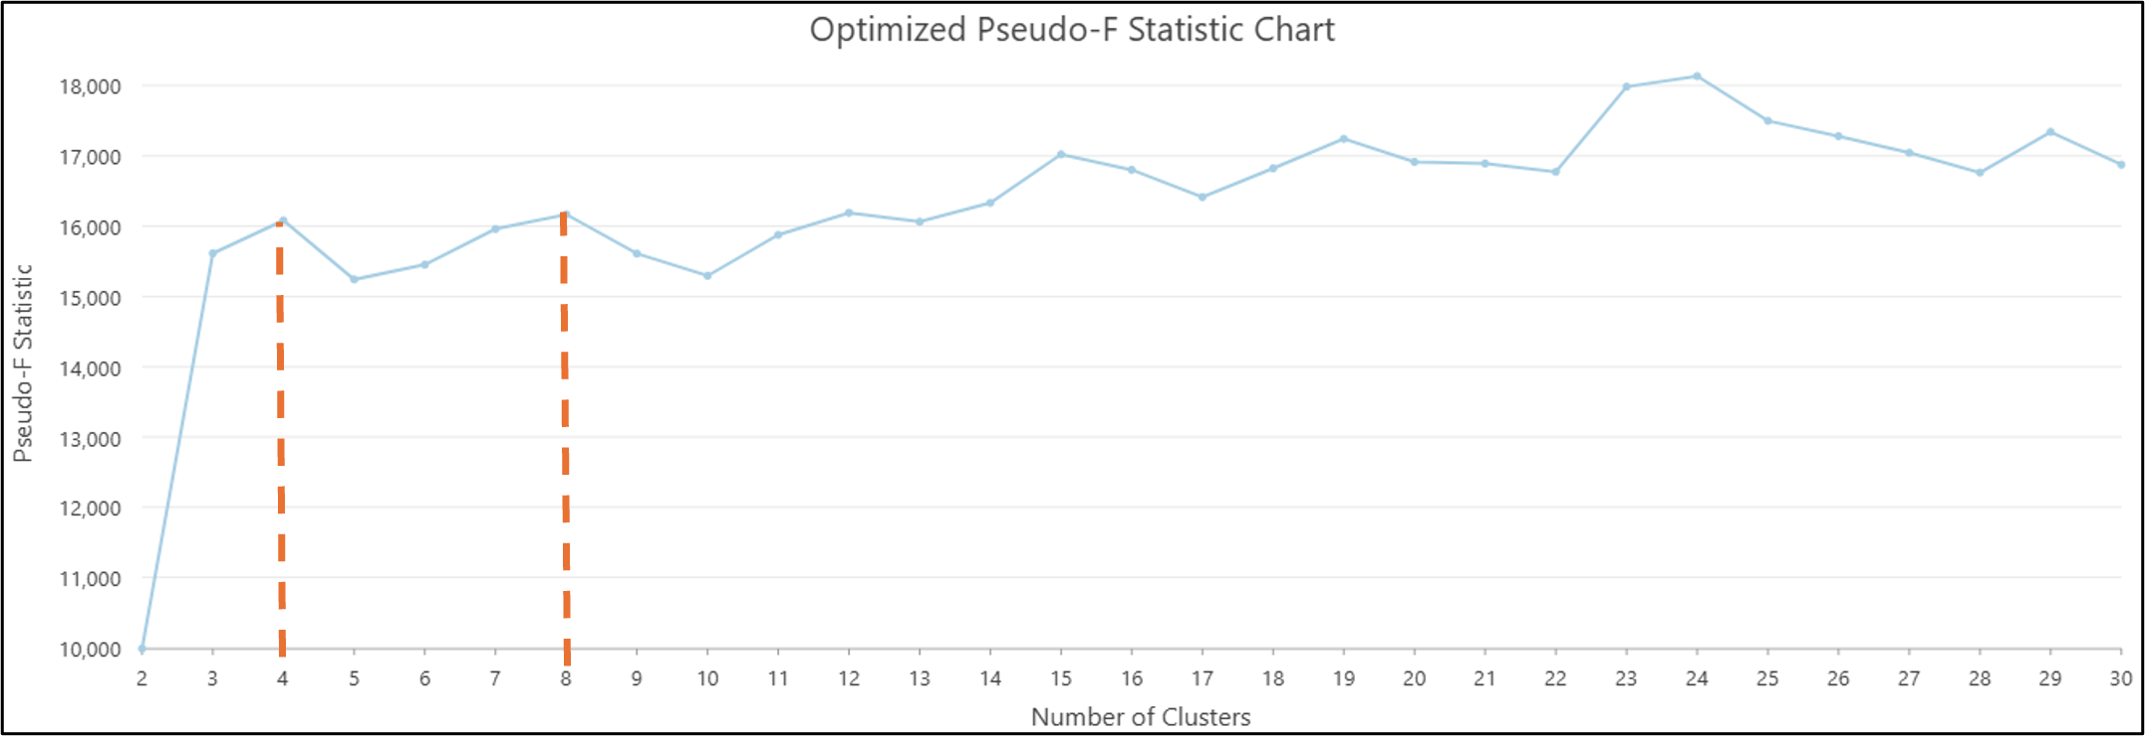
\includegraphics[keepaspectratio]{images/kmeans.png}}

  Based solely on the chart, the most appropriate number of clusters
  would be 4 or 8. In general, a larger number of clusters means that a
  smaller, more selective subset of parcels will be identified. While 8
  clusters may offer a more refined analysis and statistically stronger
  results, 4 clusters offer simplicity and ease of interpretation.

  For construction and renovation year clustering analyses, it is
  generally recommended to evaluate results from 3 to 6 clusters. This
  range should be sufficient to capture meaningful variations in housing
  characteristics while maintaining interpretability. Therefore, the
  selection of appropriate number of clusters (K) does not have to rely
  solely on statistical measures but also on the practicality of the
  resulting groups. In addition to these considerations, it is important
  to check whether the redevelopment candidates make sense when mapped
  and validated against other data such as imagery.

  The multivariate analysis may need to be run multiple times to settle
  on the most suitable number of clusters. When evaluating analysis
  outputs, it is important to verify whether each cluster represents a
  distinct and understandable housing profile based on the three fields
  of interest. ~
\item
  \textbf{Data preparation}

  Prior to running a multivariate clustering analysis, municipalities
  should translate the categorical Condition Description field into a
  new field of quantitative data, with buildings in poorer condition
  receiving lower numerical scores. Municipalities may need to evaluate
  Condition Description data in the context of their individual
  assessing standards to accurately translate them to numbers, as there
  are no statewide standards for this field. Additionally, the data may
  need to be cleaned by removing inconsistent capitalization, spelling,
  or spacing prior to creating a new field.

  Example numerical classification dictionary:

  \begin{itemize}
  \tightlist
  \item
    ``Very Poor'': 1
  \item
    ``Poor'': 2 ''
  \item
    Average-``: 3
  \item
    ``Average'': 4
  \item
    ``Average+'': 5
  \item
    ``Good'': 6
  \item
    ``Very Good'': 7
  \item
    ``Excellent'': 8
  \end{itemize}

  If the multivariate clustering tool in a municipality's software of
  choice does not automatically standardize data, it is necessary to
  standardize the EYB, AYB, and numerically transformed Condition
  Description fields due to scale differences.

  Within the Connecticut CAMA and Parcel Layer, the AYB and EYB fields
  may include null placeholder values in the form of extremely low or
  high numbers. Accordingly, municipalities should evaluate the
  distribution of these values in their CAMA data, identify any outliers
  or apparent null placeholders, verify these against their oldest
  historical buildings, and filter this data out prior to running the
  clustering analysis.

  Within the Connecticut CAMA and Parcel Layer, the AYB and EYB fields
  may include null placeholder values of 0, 15, or other extremely low
  numbers. Placeholders may also take the form of years from the 1500s,
  1600s, or 1700s. Accordingly, municipalities should evaluate the
  distribution of AYB values in their CAMA data, identify any outliers
  or apparent null placeholders, verify these against their oldest
  historical buildings, and filter this data out prior to running the
  clustering analysis.

  Example filter queries include:

  \begin{itemize}
  \tightlist
  \item
    ``EYB'' is not equal to 0
  \item
    ``EYB'' is less than or equal to 2025
  \item
    ``AYB'' is greater than or equal to 1639 (the construction year of
    the Henry Whitfield House, the oldest standing building in
    Connecticut)
  \item
    ``AYB'' \textgreater= 1788 (the year of Connecticut's founding as a
    state)
  \item
    ``AYB'' \textgreater= 1899 (a common placeholder year, as it is the
    zero date in systems like SQL, Power BI, and SharePoint)
  \end{itemize}
\item
  \textbf{Interpreting results}

  Below is a sample series of boxplots automatically produced by running
  the Multivariate Clustering tool in ArcGIS Pro. These boxplots
  illustrate the distribution of data for the three fields of interest,
  as well as which clusters contain the combination of traits most
  relevant to this analysis.

  The red line, indicating cluster 2, reveals the target relationship.
  Cluster 2 contains the lowest values of EYB and numerically
  transformed Condition Description, as well as values of AYB below the
  median. In this case, the parcels in cluster 2 would be isolated and
  included in a Potentially Redevelopable Land inventory.

  \pandocbounded{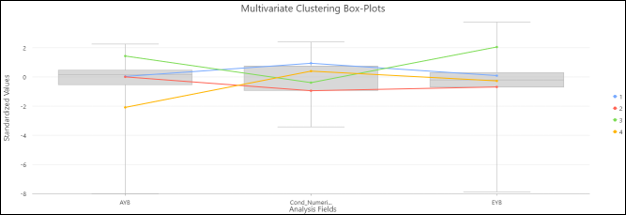
\includegraphics[keepaspectratio]{images/mc_boxplot.png}}

  Note that AYB will naturally contain lower values than EYB, as it
  reflects original construction rather than effective age.
  Additionally, the oldest buildings may have already undergone
  extensive renovation and may not exhibit similarly low condition
  ratings or EYB. Therefore, the numerically transformed Condition
  Description and EYB fields should be weighted more heavily than AYB
  when deciding which cluster to isolate, as these variables better
  reflect the current redevelopment potential of properties.

  The figure on the left shows the results of the Multivariate
  Clustering tool in ArcGIS Pro, where cluster colors on the map
  correspond to those shown in the boxplots. The figure on the right
  shows the resulting map after isolating cluster 2, which represents
  the end product of a construction and renovation year clustering
  analysis.
\end{enumerate}

\begin{figure}

\begin{minipage}[t]{0.50\linewidth}

\begin{figure}[H]

{\centering 
\includegraphics[width=3.125in,height=\textheight,keepaspectratio,alt={multivariate clustering box plot example}]{maps/MultiVar.png}

}

\subcaption{Multivariate Clustering results}

\end{figure}%

\end{minipage}%
%
\begin{minipage}[t]{0.50\linewidth}

\begin{figure}[H]

{\centering 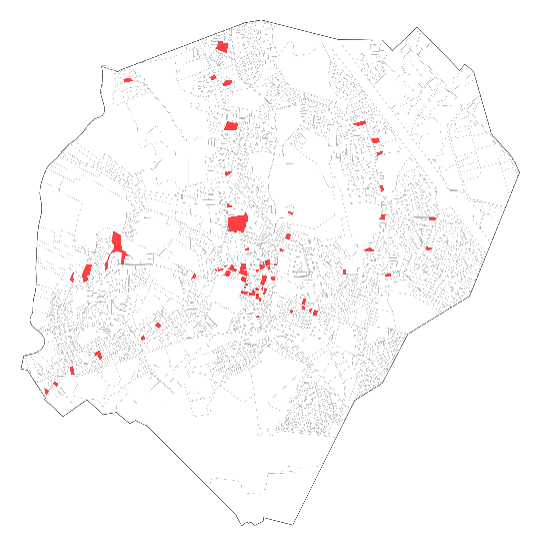
\includegraphics[width=3.125in,height=\textheight,keepaspectratio,alt={multivariate clustering box plot example}]{maps/MultiVar2.png}

}

\subcaption{Cluster 2 isolated}

\end{figure}%

\end{minipage}%

\end{figure}%

\bookmarksetup{startatroot}

\chapter{Creating the Maps}\label{creating-the-maps}

The developable land inventory analysis is a required plan element of
the Housing Growth Plan. It is not a required element of the Regional
Needs Assessment. The Guidelines recommend that this analysis be
presented through a combination of maps and narrative, and this section
focuses on the maps used to present that analysis in the Housing Growth
Plans.

The developable land inventory process is a preliminary planning-level
screening product. It is primarily analytical in nature, involving the
identification and documentation of qualifying areas through the
application of knowledge, data, and methodology. \textbf{A map is not
the mechanism by which developable areas are identified, nor does it
constitute a determination of a property's development potential}.
Rather, it serves as a visual representation of the underlying analysis,
allowing the results to be verified and understood spatially.

To support Housing Growth Plan reporting and review, the developable
land inventory should be presented in the report as municipality-wide
maps. The maps should clearly display the location and distribution of
developable land using clear, accessible, and consistent symbology.

The maps should incorporate the following data:

\begin{itemize}
\tightlist
\item
  Identified land per the statutory definitions
  (\hyperref[sec-statutory-exclusions]{Section 3})
\item
  Identified vacant parcels
  (\hyperref[identifying-vacant-and-potential-land-for-redevelopment]{Section
  4})
\item
  Identified parcels with redevelopment potential
  (\hyperref[identifying-vacant-and-potential-land-for-redevelopment]{Section
  4})
\end{itemize}

At a minimum, the following maps should be included in the Housing
Growth Plan:

\begin{enumerate}
\def\labelenumi{\arabic{enumi}.}
\item
  \textbf{Statutory Exclusions Map}: A municipality-wide map displaying
  each statutory exclusion category as a separate layer and symbolized
  distinctly to illustrate the distribution of land excluded from the
  developable land inventory, per the statutes.
\item
  \textbf{Developable Land Map}: A municipality-wide map depicting all
  land that meets the statutory definitions of developable land, shown
  as a single consolidated layer. Land excluded under the statutory
  definitions, or otherwise deemed commercially infeasible to develop,
  is shown as a separate consolidated layer. Together, these layers
  provide a simplified representation of land suitability across the
  municipality for purposes of this planning analysis.
\item
  \textbf{Developable Land Summary Map}: A municipality-wide map
  displaying land deemed developable for this planning analysis,
  alongside land excluded under the statutory definitions or otherwise
  deemed infeasible to develop, each shown as a separate consolidated
  layer. Identified vacant parcels and parcels with redevelopment
  potential should be displayed as separate overlays.
\end{enumerate}

\section{Map Layers and Symbology}\label{map-layers-and-symbology}

The following mapping standards should be applied for all final maps
included in the report. Any deviations should be explained in a brief
narrative detailing what was changed and why. Adherence to these
standards ensures consistency across all 169 municipalities statewide.

All maps include the municipal boundary layer to delineate the
geographic extent of the study area.

\textbf{Dataset}:
\href{https://geodata.ct.gov/datasets/ctmaps::ct-municipalities-with-fips/about}{CT
Municipalities (CT Geodata Portal)}

Municipal parcel boundaries may be included where appropriate to provide
spatial context for interpretation of mapped datasets.

\textbf{Dataset}:
\href{https://geodata.ct.gov/datasets/ctmaps::connecticut-cama-and-parcel-layer/about}{Connecticut
CAMA and Parcel Layer (CT Geodata Portal)}

\subsection{Map Elements}\label{map-elements}

All maps should include:

\begin{itemize}
\tightlist
\item
  Municipality-wide extent
\item
  Clear map title
\item
  Municipality name
\item
  Legend identifying all mapped categories
\item
  \hyperref[note-on-intended-use]{Note on Intended Use}, clarifying that
  the map is a planning-level screening product and not a legal or
  parcel-specific determination of development potential
\end{itemize}

\subsection{Note on Intended Use}\label{note-on-intended-use}

Each map should include a brief note clarifying the purpose and
limitations of the developable land inventory. This helps ensure that
the map is not misread as a legal or parcel-specific determination of
development potential. Municipalities may adjust the language below as
needed, provided the core message is retained.

\emph{Suggested language:}

\begin{quote}
This map is a planning-level screening product prepared for
{[}municipality name{]}'s developable land inventory, as required under
C.G.S. Sec. 8-13aa -- 8-13dd. It is intended for municipal planning
purposes only and does not constitute a legal or parcel-specific
determination of development potential.
\end{quote}

\subsection{Symbology}\label{symbology}

\begin{tcolorbox}[enhanced jigsaw, arc=.35mm, bottomrule=.15mm, breakable, colback=white, colframe=quarto-callout-caution-color-frame, left=2mm, leftrule=.75mm, opacityback=0, rightrule=.15mm, toprule=.15mm]

Map symbology should use colors and patterns that improve overall
readability, provide clear visual distinction between categories, and
remain accessible to users with color vision deficiencies.

\end{tcolorbox}

\begin{enumerate}
\def\labelenumi{\arabic{enumi}.}
\tightlist
\item
  \textbf{Statutory Exclusions Map}
\end{enumerate}

\global\setlength{\Oldarrayrulewidth}{\arrayrulewidth}

\global\setlength{\Oldtabcolsep}{\tabcolsep}

\setlength{\tabcolsep}{2pt}

\renewcommand*{\arraystretch}{1.5}



\providecommand{\ascline}[3]{\noalign{\global\arrayrulewidth #1}\arrayrulecolor[HTML]{#2}\cline{#3}}

\begin{longtable*}[c]{|p{1.40in}|p{1.40in}|p{1.00in}|p{1.00in}|p{0.70in}}



\ascline{1.5pt}{666666}{1-5}

\multicolumn{1}{>{\raggedright}p{\dimexpr 1.4in+0\tabcolsep}}{\advance\leftskip by 4.0pt\relax \advance\rightskip by 4.0pt\relax \textcolor[HTML]{000000}{\fontsize{10}{10}\selectfont{{\fontspec{Arial} \textbf{Map\ Layer\ (top\ to\ bottom)}}}}} & \multicolumn{1}{>{\raggedright}p{\dimexpr 1.4in+0\tabcolsep}}{\advance\leftskip by 4.0pt\relax \advance\rightskip by 4.0pt\relax \textcolor[HTML]{000000}{\fontsize{10}{10}\selectfont{{\fontspec{Arial} \textbf{Description}}}}} & \multicolumn{3}{>{\raggedright}p{\dimexpr 2.7in+4\tabcolsep}}{\advance\leftskip by 4.0pt\relax \advance\rightskip by 4.0pt\relax \textcolor[HTML]{000000}{\fontsize{10}{10}\selectfont{{\fontspec{Arial} \textbf{Symbology}}}}} \\

\ascline{0.75pt}{666666}{3-5}



\multicolumn{1}{>{\raggedright}p{\dimexpr 1.4in+0\tabcolsep}}{} & \multicolumn{1}{>{\raggedright}p{\dimexpr 1.4in+0\tabcolsep}}{} & \multicolumn{1}{>{\raggedright}p{\dimexpr 1in+0\tabcolsep}}{\advance\leftskip by 4.0pt\relax \advance\rightskip by 4.0pt\relax \textcolor[HTML]{000000}{\fontsize{10}{10}\selectfont{{\fontspec{Arial} \textbf{Fill}}}}} & \multicolumn{1}{>{\raggedright}p{\dimexpr 1in+0\tabcolsep}}{\advance\leftskip by 4.0pt\relax \advance\rightskip by 4.0pt\relax \textcolor[HTML]{000000}{\fontsize{10}{10}\selectfont{{\fontspec{Arial} \textbf{Outline}}}}} & \multicolumn{1}{>{\raggedright}p{\dimexpr 0.7in+0\tabcolsep}}{\advance\leftskip by 4.0pt\relax \advance\rightskip by 4.0pt\relax \textcolor[HTML]{000000}{\fontsize{10}{10}\selectfont{{\fontspec{Arial} \textbf{Transparency}}}}} \\

\ascline{1.5pt}{666666}{1-5}\endfirsthead 

\ascline{1.5pt}{666666}{1-5}

\multicolumn{1}{>{\raggedright}p{\dimexpr 1.4in+0\tabcolsep}}{\advance\leftskip by 4.0pt\relax \advance\rightskip by 4.0pt\relax \textcolor[HTML]{000000}{\fontsize{10}{10}\selectfont{{\fontspec{Arial} \textbf{Map\ Layer\ (top\ to\ bottom)}}}}} & \multicolumn{1}{>{\raggedright}p{\dimexpr 1.4in+0\tabcolsep}}{\advance\leftskip by 4.0pt\relax \advance\rightskip by 4.0pt\relax \textcolor[HTML]{000000}{\fontsize{10}{10}\selectfont{{\fontspec{Arial} \textbf{Description}}}}} & \multicolumn{3}{>{\raggedright}p{\dimexpr 2.7in+4\tabcolsep}}{\advance\leftskip by 4.0pt\relax \advance\rightskip by 4.0pt\relax \textcolor[HTML]{000000}{\fontsize{10}{10}\selectfont{{\fontspec{Arial} \textbf{Symbology}}}}} \\

\ascline{0.75pt}{666666}{3-5}



\multicolumn{1}{>{\raggedright}p{\dimexpr 1.4in+0\tabcolsep}}{} & \multicolumn{1}{>{\raggedright}p{\dimexpr 1.4in+0\tabcolsep}}{} & \multicolumn{1}{>{\raggedright}p{\dimexpr 1in+0\tabcolsep}}{\advance\leftskip by 4.0pt\relax \advance\rightskip by 4.0pt\relax \textcolor[HTML]{000000}{\fontsize{10}{10}\selectfont{{\fontspec{Arial} \textbf{Fill}}}}} & \multicolumn{1}{>{\raggedright}p{\dimexpr 1in+0\tabcolsep}}{\advance\leftskip by 4.0pt\relax \advance\rightskip by 4.0pt\relax \textcolor[HTML]{000000}{\fontsize{10}{10}\selectfont{{\fontspec{Arial} \textbf{Outline}}}}} & \multicolumn{1}{>{\raggedright}p{\dimexpr 0.7in+0\tabcolsep}}{\advance\leftskip by 4.0pt\relax \advance\rightskip by 4.0pt\relax \textcolor[HTML]{000000}{\fontsize{10}{10}\selectfont{{\fontspec{Arial} \textbf{Transparency}}}}} \\

\ascline{1.5pt}{666666}{1-5}\endhead



\multicolumn{1}{>{\raggedright}p{\dimexpr 1.4in+0\tabcolsep}}{\advance\leftskip by 4.0pt\relax \advance\rightskip by 4.0pt\relax \textcolor[HTML]{000000}{\fontsize{10}{10}\selectfont{{\fontspec{Arial} Municipality\ boundary}}}} & \multicolumn{1}{>{\raggedright}p{\dimexpr 1.4in+0\tabcolsep}}{\advance\leftskip by 4.0pt\relax \advance\rightskip by 4.0pt\relax \textcolor[HTML]{000000}{\fontsize{10}{10}\selectfont{{\fontspec{Arial} Municipal\ boundary\ delineating\ the\ extent\ of\ the\ study\ area}}}} & \multicolumn{1}{>{\raggedright}p{\dimexpr 1in+0\tabcolsep}}{\advance\leftskip by 4.0pt\relax \advance\rightskip by 4.0pt\relax \textcolor[HTML]{000000}{\fontsize{10}{10}\selectfont{{\fontspec{Arial} None}}}} & \multicolumn{1}{>{\raggedright}p{\dimexpr 1in+0\tabcolsep}}{\advance\leftskip by 4.0pt\relax \advance\rightskip by 4.0pt\relax \textcolor[HTML]{000000}{\fontsize{10}{10}\selectfont{{\fontspec{Arial} 0.6\ pt,}}}\textcolor[HTML]{000000}{\fontsize{10}{10}\selectfont{{\fontspec{Arial} \linebreak }}}\textcolor[HTML]{000000}{\fontsize{10}{10}\selectfont{{\fontspec{Arial} Dark\ gray}}}\textcolor[HTML]{000000}{\fontsize{10}{10}\selectfont{{\fontspec{Arial} \linebreak }}}\textcolor[HTML]{000000}{\fontsize{10}{10}\selectfont{{\fontspec{Arial} (\#343434)}}}} & \multicolumn{1}{>{\raggedright}p{\dimexpr 0.7in+0\tabcolsep}}{\advance\leftskip by 4.0pt\relax \advance\rightskip by 4.0pt\relax \textcolor[HTML]{000000}{\fontsize{10}{10}\selectfont{{\fontspec{Arial} 0\%}}}} \\

\ascline{0.75pt}{666666}{1-5}



\multicolumn{1}{>{\raggedright}p{\dimexpr 1.4in+0\tabcolsep}}{\advance\leftskip by 4.0pt\relax \advance\rightskip by 4.0pt\relax \textcolor[HTML]{000000}{\fontsize{10}{10}\selectfont{{\fontspec{Arial} Parcels}}}} & \multicolumn{1}{>{\raggedright}p{\dimexpr 1.4in+0\tabcolsep}}{\advance\leftskip by 4.0pt\relax \advance\rightskip by 4.0pt\relax \textcolor[HTML]{000000}{\fontsize{10}{10}\selectfont{{\fontspec{Arial} Municipal\ parcel\ boundaries,\ used\ only\ for\ visual\ context}}}} & \multicolumn{1}{>{\raggedright}p{\dimexpr 1in+0\tabcolsep}}{\advance\leftskip by 4.0pt\relax \advance\rightskip by 4.0pt\relax \textcolor[HTML]{000000}{\fontsize{10}{10}\selectfont{{\fontspec{Arial} None}}}} & \multicolumn{1}{>{\raggedright}p{\dimexpr 1in+0\tabcolsep}}{\advance\leftskip by 4.0pt\relax \advance\rightskip by 4.0pt\relax \textcolor[HTML]{000000}{\fontsize{10}{10}\selectfont{{\fontspec{Arial} 0.1\ pt,}}}\textcolor[HTML]{000000}{\fontsize{10}{10}\selectfont{{\fontspec{Arial} \linebreak }}}\textcolor[HTML]{000000}{\fontsize{10}{10}\selectfont{{\fontspec{Arial} Dark\ gray}}}\textcolor[HTML]{000000}{\fontsize{10}{10}\selectfont{{\fontspec{Arial} \linebreak }}}\textcolor[HTML]{000000}{\fontsize{10}{10}\selectfont{{\fontspec{Arial} (\#343434)}}}} & \multicolumn{1}{>{\raggedright}p{\dimexpr 0.7in+0\tabcolsep}}{\advance\leftskip by 4.0pt\relax \advance\rightskip by 4.0pt\relax \textcolor[HTML]{000000}{\fontsize{10}{10}\selectfont{{\fontspec{Arial} 30\%}}}} \\

\ascline{0.75pt}{666666}{1-5}



\multicolumn{1}{>{\raggedright}p{\dimexpr 1.4in+0\tabcolsep}}{\advance\leftskip by 4.0pt\relax \advance\rightskip by 4.0pt\relax \textcolor[HTML]{000000}{\fontsize{10}{10}\selectfont{{\fontspec{Arial} Land\ subject\ to\ enforceable\ restrictions\ or\ prohibitions\ on\ development}}}} & \multicolumn{1}{>{\raggedright}p{\dimexpr 1.4in+0\tabcolsep}}{\advance\leftskip by 4.0pt\relax \advance\rightskip by 4.0pt\relax \textcolor[HTML]{000000}{\fontsize{10}{10}\selectfont{{\fontspec{Arial} Exclusion\ category\ described\ in\ Section\ 3.3}}}} & \multicolumn{1}{>{\raggedright}p{\dimexpr 1in+0\tabcolsep}}{\advance\leftskip by 4.0pt\relax \advance\rightskip by 4.0pt\relax \textcolor[HTML]{000000}{\fontsize{10}{10}\selectfont{{\fontspec{Arial} Hatched\ \&\ Solid,}}}\textcolor[HTML]{000000}{\fontsize{10}{10}\selectfont{{\fontspec{Arial} \linebreak }}}\textcolor[HTML]{000000}{\fontsize{10}{10}\selectfont{{\fontspec{Arial} Red}}}\textcolor[HTML]{000000}{\fontsize{10}{10}\selectfont{{\fontspec{Arial} \linebreak }}}\textcolor[HTML]{000000}{\fontsize{10}{10}\selectfont{{\fontspec{Arial} (\#FF0000)}}}} & \multicolumn{1}{>{\raggedright}p{\dimexpr 1in+0\tabcolsep}}{\advance\leftskip by 4.0pt\relax \advance\rightskip by 4.0pt\relax \textcolor[HTML]{000000}{\fontsize{10}{10}\selectfont{{\fontspec{Arial} None}}}} & \multicolumn{1}{>{\raggedright}p{\dimexpr 0.7in+0\tabcolsep}}{\advance\leftskip by 4.0pt\relax \advance\rightskip by 4.0pt\relax \textcolor[HTML]{000000}{\fontsize{10}{10}\selectfont{{\fontspec{Arial} 0\%\ hatch\ lines,}}}\textcolor[HTML]{000000}{\fontsize{10}{10}\selectfont{{\fontspec{Arial} \linebreak }}}\textcolor[HTML]{000000}{\fontsize{10}{10}\selectfont{{\fontspec{Arial} \ 75\%\ solid\ fill}}}} \\

\ascline{0.75pt}{666666}{1-5}



\multicolumn{1}{>{\raggedright}p{\dimexpr 1.4in+0\tabcolsep}}{\advance\leftskip by 4.0pt\relax \advance\rightskip by 4.0pt\relax \textcolor[HTML]{000000}{\fontsize{10}{10}\selectfont{{\fontspec{Arial} Land\ already\ committed\ to\ public\ use\ or\ purpose}}}} & \multicolumn{1}{>{\raggedright}p{\dimexpr 1.4in+0\tabcolsep}}{\advance\leftskip by 4.0pt\relax \advance\rightskip by 4.0pt\relax \textcolor[HTML]{000000}{\fontsize{10}{10}\selectfont{{\fontspec{Arial} Exclusion\ category\ described\ in\ Section\ 3.1}}}} & \multicolumn{1}{>{\raggedright}p{\dimexpr 1in+0\tabcolsep}}{\advance\leftskip by 4.0pt\relax \advance\rightskip by 4.0pt\relax \textcolor[HTML]{000000}{\fontsize{10}{10}\selectfont{{\fontspec{Arial} Solid,}}}\textcolor[HTML]{000000}{\fontsize{10}{10}\selectfont{{\fontspec{Arial} \linebreak }}}\textcolor[HTML]{000000}{\fontsize{10}{10}\selectfont{{\fontspec{Arial} Dark\ orange}}}\textcolor[HTML]{000000}{\fontsize{10}{10}\selectfont{{\fontspec{Arial} \linebreak }}}\textcolor[HTML]{000000}{\fontsize{10}{10}\selectfont{{\fontspec{Arial} (\#CC5629)}}}} & \multicolumn{1}{>{\raggedright}p{\dimexpr 1in+0\tabcolsep}}{\advance\leftskip by 4.0pt\relax \advance\rightskip by 4.0pt\relax \textcolor[HTML]{000000}{\fontsize{10}{10}\selectfont{{\fontspec{Arial} None}}}} & \multicolumn{1}{>{\raggedright}p{\dimexpr 0.7in+0\tabcolsep}}{\advance\leftskip by 4.0pt\relax \advance\rightskip by 4.0pt\relax \textcolor[HTML]{000000}{\fontsize{10}{10}\selectfont{{\fontspec{Arial} 20\%}}}} \\

\ascline{0.75pt}{666666}{1-5}



\multicolumn{1}{>{\raggedright}p{\dimexpr 1.4in+0\tabcolsep}}{\advance\leftskip by 4.0pt\relax \advance\rightskip by 4.0pt\relax \textcolor[HTML]{000000}{\fontsize{10}{10}\selectfont{{\fontspec{Arial} Open\ space,\ parks,\ and\ recreation\ areas\ dedicated\ to\ the\ public\ or\ protected\ by\ a\ conservation\ easement}}}} & \multicolumn{1}{>{\raggedright}p{\dimexpr 1.4in+0\tabcolsep}}{\advance\leftskip by 4.0pt\relax \advance\rightskip by 4.0pt\relax \textcolor[HTML]{000000}{\fontsize{10}{10}\selectfont{{\fontspec{Arial} Exclusion\ category\ described\ in\ Section\ 3.2}}}} & \multicolumn{1}{>{\raggedright}p{\dimexpr 1in+0\tabcolsep}}{\advance\leftskip by 4.0pt\relax \advance\rightskip by 4.0pt\relax \textcolor[HTML]{000000}{\fontsize{10}{10}\selectfont{{\fontspec{Arial} Solid,}}}\textcolor[HTML]{000000}{\fontsize{10}{10}\selectfont{{\fontspec{Arial} \linebreak }}}\textcolor[HTML]{000000}{\fontsize{10}{10}\selectfont{{\fontspec{Arial} Medium\ yellow}}}\textcolor[HTML]{000000}{\fontsize{10}{10}\selectfont{{\fontspec{Arial} \linebreak }}}\textcolor[HTML]{000000}{\fontsize{10}{10}\selectfont{{\fontspec{Arial} (\#F9AB34)}}}} & \multicolumn{1}{>{\raggedright}p{\dimexpr 1in+0\tabcolsep}}{\advance\leftskip by 4.0pt\relax \advance\rightskip by 4.0pt\relax \textcolor[HTML]{000000}{\fontsize{10}{10}\selectfont{{\fontspec{Arial} None}}}} & \multicolumn{1}{>{\raggedright}p{\dimexpr 0.7in+0\tabcolsep}}{\advance\leftskip by 4.0pt\relax \advance\rightskip by 4.0pt\relax \textcolor[HTML]{000000}{\fontsize{10}{10}\selectfont{{\fontspec{Arial} 20\%}}}} \\

\ascline{0.75pt}{666666}{1-5}



\multicolumn{1}{>{\raggedright}p{\dimexpr 1.4in+0\tabcolsep}}{\advance\leftskip by 4.0pt\relax \advance\rightskip by 4.0pt\relax \textcolor[HTML]{000000}{\fontsize{10}{10}\selectfont{{\fontspec{Arial} Areas\ of\ 0.5\ acres\ or\ more\ of\ contiguous\ land\ that\ are\ unsuitable\ for\ development\ due\ to\ topography\ (such\ as\ steep\ slopes)}}}} & \multicolumn{1}{>{\raggedright}p{\dimexpr 1.4in+0\tabcolsep}}{\advance\leftskip by 4.0pt\relax \advance\rightskip by 4.0pt\relax \textcolor[HTML]{000000}{\fontsize{10}{10}\selectfont{{\fontspec{Arial} Exclusion\ category\ described\ in\ Section\ 3.5}}}} & \multicolumn{1}{>{\raggedright}p{\dimexpr 1in+0\tabcolsep}}{\advance\leftskip by 4.0pt\relax \advance\rightskip by 4.0pt\relax \textcolor[HTML]{000000}{\fontsize{10}{10}\selectfont{{\fontspec{Arial} Solid,}}}\textcolor[HTML]{000000}{\fontsize{10}{10}\selectfont{{\fontspec{Arial} \linebreak }}}\textcolor[HTML]{000000}{\fontsize{10}{10}\selectfont{{\fontspec{Arial} Brown}}}\textcolor[HTML]{000000}{\fontsize{10}{10}\selectfont{{\fontspec{Arial} \linebreak }}}\textcolor[HTML]{000000}{\fontsize{10}{10}\selectfont{{\fontspec{Arial} (\#664F3C)}}}} & \multicolumn{1}{>{\raggedright}p{\dimexpr 1in+0\tabcolsep}}{\advance\leftskip by 4.0pt\relax \advance\rightskip by 4.0pt\relax \textcolor[HTML]{000000}{\fontsize{10}{10}\selectfont{{\fontspec{Arial} None}}}} & \multicolumn{1}{>{\raggedright}p{\dimexpr 0.7in+0\tabcolsep}}{\advance\leftskip by 4.0pt\relax \advance\rightskip by 4.0pt\relax \textcolor[HTML]{000000}{\fontsize{10}{10}\selectfont{{\fontspec{Arial} 15\%}}}} \\

\ascline{0.75pt}{666666}{1-5}



\multicolumn{1}{>{\raggedright}p{\dimexpr 1.4in+0\tabcolsep}}{\advance\leftskip by 4.0pt\relax \advance\rightskip by 4.0pt\relax \textcolor[HTML]{000000}{\fontsize{10}{10}\selectfont{{\fontspec{Arial} Wetlands\ or\ watercourses,\ as\ defined\ in\ the\ Wetlands\ and\ Watercourses\ Act\ (CGS\ Chapter\ 440)}}}} & \multicolumn{1}{>{\raggedright}p{\dimexpr 1.4in+0\tabcolsep}}{\advance\leftskip by 4.0pt\relax \advance\rightskip by 4.0pt\relax \textcolor[HTML]{000000}{\fontsize{10}{10}\selectfont{{\fontspec{Arial} Exclusion\ category\ described\ in\ Section\ 3.4}}}} & \multicolumn{1}{>{\raggedright}p{\dimexpr 1in+0\tabcolsep}}{\advance\leftskip by 4.0pt\relax \advance\rightskip by 4.0pt\relax \textcolor[HTML]{000000}{\fontsize{10}{10}\selectfont{{\fontspec{Arial} Solid,}}}\textcolor[HTML]{000000}{\fontsize{10}{10}\selectfont{{\fontspec{Arial} \linebreak }}}\textcolor[HTML]{000000}{\fontsize{10}{10}\selectfont{{\fontspec{Arial} Medium\ blue}}}\textcolor[HTML]{000000}{\fontsize{10}{10}\selectfont{{\fontspec{Arial} \linebreak }}}\textcolor[HTML]{000000}{\fontsize{10}{10}\selectfont{{\fontspec{Arial} (\#0070FF)}}}} & \multicolumn{1}{>{\raggedright}p{\dimexpr 1in+0\tabcolsep}}{\advance\leftskip by 4.0pt\relax \advance\rightskip by 4.0pt\relax \textcolor[HTML]{000000}{\fontsize{10}{10}\selectfont{{\fontspec{Arial} None}}}} & \multicolumn{1}{>{\raggedright}p{\dimexpr 0.7in+0\tabcolsep}}{\advance\leftskip by 4.0pt\relax \advance\rightskip by 4.0pt\relax \textcolor[HTML]{000000}{\fontsize{10}{10}\selectfont{{\fontspec{Arial} 40\%}}}} \\

\ascline{1.5pt}{666666}{1-5}



\end{longtable*}



\arrayrulecolor[HTML]{000000}

\global\setlength{\arrayrulewidth}{\Oldarrayrulewidth}

\global\setlength{\tabcolsep}{\Oldtabcolsep}

\renewcommand*{\arraystretch}{1}

\begin{figure}[H]

{\centering \pandocbounded{\includegraphics[keepaspectratio,alt={Example Statutory Exclusions Map}]{maps/excl_map_bordered.png}}

}

\caption{\emph{Example Statutory Exclusions Map}
\href{https://github.com/ctgisoffice/dev-land-inv-guidance/blob/master/maps/excl.png?raw=true}{View
full-size map}}

\end{figure}%

\begin{enumerate}
\def\labelenumi{\arabic{enumi}.}
\setcounter{enumi}{1}
\tightlist
\item
  \textbf{Developable Land Map}
\end{enumerate}

\global\setlength{\Oldarrayrulewidth}{\arrayrulewidth}

\global\setlength{\Oldtabcolsep}{\tabcolsep}

\setlength{\tabcolsep}{2pt}

\renewcommand*{\arraystretch}{1.5}



\providecommand{\ascline}[3]{\noalign{\global\arrayrulewidth #1}\arrayrulecolor[HTML]{#2}\cline{#3}}

\begin{longtable*}[c]{|p{1.40in}|p{1.40in}|p{1.00in}|p{1.00in}|p{0.70in}}



\ascline{1.5pt}{666666}{1-5}

\multicolumn{1}{>{\raggedright}p{\dimexpr 1.4in+0\tabcolsep}}{\advance\leftskip by 4.0pt\relax \advance\rightskip by 4.0pt\relax \textcolor[HTML]{000000}{\fontsize{10}{10}\selectfont{{\fontspec{Arial} \textbf{Map\ Layer\ (top\ to\ bottom)}}}}} & \multicolumn{1}{>{\raggedright}p{\dimexpr 1.4in+0\tabcolsep}}{\advance\leftskip by 4.0pt\relax \advance\rightskip by 4.0pt\relax \textcolor[HTML]{000000}{\fontsize{10}{10}\selectfont{{\fontspec{Arial} \textbf{Description}}}}} & \multicolumn{3}{>{\raggedright}p{\dimexpr 2.7in+4\tabcolsep}}{\advance\leftskip by 4.0pt\relax \advance\rightskip by 4.0pt\relax \textcolor[HTML]{000000}{\fontsize{10}{10}\selectfont{{\fontspec{Arial} \textbf{Symbology}}}}} \\

\ascline{0.75pt}{666666}{3-5}



\multicolumn{1}{>{\raggedright}p{\dimexpr 1.4in+0\tabcolsep}}{} & \multicolumn{1}{>{\raggedright}p{\dimexpr 1.4in+0\tabcolsep}}{} & \multicolumn{1}{>{\raggedright}p{\dimexpr 1in+0\tabcolsep}}{\advance\leftskip by 4.0pt\relax \advance\rightskip by 4.0pt\relax \textcolor[HTML]{000000}{\fontsize{10}{10}\selectfont{{\fontspec{Arial} \textbf{Fill}}}}} & \multicolumn{1}{>{\raggedright}p{\dimexpr 1in+0\tabcolsep}}{\advance\leftskip by 4.0pt\relax \advance\rightskip by 4.0pt\relax \textcolor[HTML]{000000}{\fontsize{10}{10}\selectfont{{\fontspec{Arial} \textbf{Outline}}}}} & \multicolumn{1}{>{\raggedright}p{\dimexpr 0.7in+0\tabcolsep}}{\advance\leftskip by 4.0pt\relax \advance\rightskip by 4.0pt\relax \textcolor[HTML]{000000}{\fontsize{10}{10}\selectfont{{\fontspec{Arial} \textbf{Transparency}}}}} \\

\ascline{1.5pt}{666666}{1-5}\endfirsthead 

\ascline{1.5pt}{666666}{1-5}

\multicolumn{1}{>{\raggedright}p{\dimexpr 1.4in+0\tabcolsep}}{\advance\leftskip by 4.0pt\relax \advance\rightskip by 4.0pt\relax \textcolor[HTML]{000000}{\fontsize{10}{10}\selectfont{{\fontspec{Arial} \textbf{Map\ Layer\ (top\ to\ bottom)}}}}} & \multicolumn{1}{>{\raggedright}p{\dimexpr 1.4in+0\tabcolsep}}{\advance\leftskip by 4.0pt\relax \advance\rightskip by 4.0pt\relax \textcolor[HTML]{000000}{\fontsize{10}{10}\selectfont{{\fontspec{Arial} \textbf{Description}}}}} & \multicolumn{3}{>{\raggedright}p{\dimexpr 2.7in+4\tabcolsep}}{\advance\leftskip by 4.0pt\relax \advance\rightskip by 4.0pt\relax \textcolor[HTML]{000000}{\fontsize{10}{10}\selectfont{{\fontspec{Arial} \textbf{Symbology}}}}} \\

\ascline{0.75pt}{666666}{3-5}



\multicolumn{1}{>{\raggedright}p{\dimexpr 1.4in+0\tabcolsep}}{} & \multicolumn{1}{>{\raggedright}p{\dimexpr 1.4in+0\tabcolsep}}{} & \multicolumn{1}{>{\raggedright}p{\dimexpr 1in+0\tabcolsep}}{\advance\leftskip by 4.0pt\relax \advance\rightskip by 4.0pt\relax \textcolor[HTML]{000000}{\fontsize{10}{10}\selectfont{{\fontspec{Arial} \textbf{Fill}}}}} & \multicolumn{1}{>{\raggedright}p{\dimexpr 1in+0\tabcolsep}}{\advance\leftskip by 4.0pt\relax \advance\rightskip by 4.0pt\relax \textcolor[HTML]{000000}{\fontsize{10}{10}\selectfont{{\fontspec{Arial} \textbf{Outline}}}}} & \multicolumn{1}{>{\raggedright}p{\dimexpr 0.7in+0\tabcolsep}}{\advance\leftskip by 4.0pt\relax \advance\rightskip by 4.0pt\relax \textcolor[HTML]{000000}{\fontsize{10}{10}\selectfont{{\fontspec{Arial} \textbf{Transparency}}}}} \\

\ascline{1.5pt}{666666}{1-5}\endhead



\multicolumn{1}{>{\raggedright}p{\dimexpr 1.4in+0\tabcolsep}}{\advance\leftskip by 4.0pt\relax \advance\rightskip by 4.0pt\relax \textcolor[HTML]{000000}{\fontsize{10}{10}\selectfont{{\fontspec{Arial} Municipality\ boundary}}}} & \multicolumn{1}{>{\raggedright}p{\dimexpr 1.4in+0\tabcolsep}}{\advance\leftskip by 4.0pt\relax \advance\rightskip by 4.0pt\relax \textcolor[HTML]{000000}{\fontsize{10}{10}\selectfont{{\fontspec{Arial} Municipal\ boundary\ delineating\ the\ extent\ of\ the\ study\ area.}}}} & \multicolumn{1}{>{\raggedright}p{\dimexpr 1in+0\tabcolsep}}{\advance\leftskip by 4.0pt\relax \advance\rightskip by 4.0pt\relax \textcolor[HTML]{000000}{\fontsize{10}{10}\selectfont{{\fontspec{Arial} None}}}} & \multicolumn{1}{>{\raggedright}p{\dimexpr 1in+0\tabcolsep}}{\advance\leftskip by 4.0pt\relax \advance\rightskip by 4.0pt\relax \textcolor[HTML]{000000}{\fontsize{10}{10}\selectfont{{\fontspec{Arial} 0.6\ pt,}}}\textcolor[HTML]{000000}{\fontsize{10}{10}\selectfont{{\fontspec{Arial} \linebreak }}}\textcolor[HTML]{000000}{\fontsize{10}{10}\selectfont{{\fontspec{Arial} Dark\ gray}}}\textcolor[HTML]{000000}{\fontsize{10}{10}\selectfont{{\fontspec{Arial} \linebreak }}}\textcolor[HTML]{000000}{\fontsize{10}{10}\selectfont{{\fontspec{Arial} (\#343434)}}}} & \multicolumn{1}{>{\raggedright}p{\dimexpr 0.7in+0\tabcolsep}}{\advance\leftskip by 4.0pt\relax \advance\rightskip by 4.0pt\relax \textcolor[HTML]{000000}{\fontsize{10}{10}\selectfont{{\fontspec{Arial} 0\%}}}} \\

\ascline{0.75pt}{666666}{1-5}



\multicolumn{1}{>{\raggedright}p{\dimexpr 1.4in+0\tabcolsep}}{\advance\leftskip by 4.0pt\relax \advance\rightskip by 4.0pt\relax \textcolor[HTML]{000000}{\fontsize{10}{10}\selectfont{{\fontspec{Arial} Statutory\ exclusions}}}} & \multicolumn{1}{>{\raggedright}p{\dimexpr 1.4in+0\tabcolsep}}{\advance\leftskip by 4.0pt\relax \advance\rightskip by 4.0pt\relax \textcolor[HTML]{000000}{\fontsize{10}{10}\selectfont{{\fontspec{Arial} Areas\ excluded\ from\ the\ developable\ land\ inventory\ (not\ commerically\ feasible\ and/or\ meet\ statutory\ exclusion\ categories\ from\ Section\ 3).\ Combined\ into\ a\ single\ layer.}}}} & \multicolumn{1}{>{\raggedright}p{\dimexpr 1in+0\tabcolsep}}{\advance\leftskip by 4.0pt\relax \advance\rightskip by 4.0pt\relax \textcolor[HTML]{000000}{\fontsize{10}{10}\selectfont{{\fontspec{Arial} Solid,}}}\textcolor[HTML]{000000}{\fontsize{10}{10}\selectfont{{\fontspec{Arial} \linebreak }}}\textcolor[HTML]{000000}{\fontsize{10}{10}\selectfont{{\fontspec{Arial} Dark\ gray}}}\textcolor[HTML]{000000}{\fontsize{10}{10}\selectfont{{\fontspec{Arial} \linebreak }}}\textcolor[HTML]{000000}{\fontsize{10}{10}\selectfont{{\fontspec{Arial} (\#4E4E4E)}}}} & \multicolumn{1}{>{\raggedright}p{\dimexpr 1in+0\tabcolsep}}{\advance\leftskip by 4.0pt\relax \advance\rightskip by 4.0pt\relax \textcolor[HTML]{000000}{\fontsize{10}{10}\selectfont{{\fontspec{Arial} None}}}} & \multicolumn{1}{>{\raggedright}p{\dimexpr 0.7in+0\tabcolsep}}{\advance\leftskip by 4.0pt\relax \advance\rightskip by 4.0pt\relax \textcolor[HTML]{000000}{\fontsize{10}{10}\selectfont{{\fontspec{Arial} 0\%}}}} \\

\ascline{0.75pt}{666666}{1-5}



\multicolumn{1}{>{\raggedright}p{\dimexpr 1.4in+0\tabcolsep}}{\advance\leftskip by 4.0pt\relax \advance\rightskip by 4.0pt\relax \textcolor[HTML]{000000}{\fontsize{10}{10}\selectfont{{\fontspec{Arial} Developable\ land}}}} & \multicolumn{1}{>{\raggedright}p{\dimexpr 1.4in+0\tabcolsep}}{\advance\leftskip by 4.0pt\relax \advance\rightskip by 4.0pt\relax \textcolor[HTML]{000000}{\fontsize{10}{10}\selectfont{{\fontspec{Arial} Land\ deemed\ developable\ per\ the\ statutory\ definitions.\ Combined\ into\ a\ single\ layer.}}}} & \multicolumn{1}{>{\raggedright}p{\dimexpr 1in+0\tabcolsep}}{\advance\leftskip by 4.0pt\relax \advance\rightskip by 4.0pt\relax \textcolor[HTML]{000000}{\fontsize{10}{10}\selectfont{{\fontspec{Arial} Solid,}}}\textcolor[HTML]{000000}{\fontsize{10}{10}\selectfont{{\fontspec{Arial} \linebreak }}}\textcolor[HTML]{000000}{\fontsize{10}{10}\selectfont{{\fontspec{Arial} Light\ gray}}}\textcolor[HTML]{000000}{\fontsize{10}{10}\selectfont{{\fontspec{Arial} \linebreak }}}\textcolor[HTML]{000000}{\fontsize{10}{10}\selectfont{{\fontspec{Arial} (\#E1E1E1)}}}} & \multicolumn{1}{>{\raggedright}p{\dimexpr 1in+0\tabcolsep}}{\advance\leftskip by 4.0pt\relax \advance\rightskip by 4.0pt\relax \textcolor[HTML]{000000}{\fontsize{10}{10}\selectfont{{\fontspec{Arial} None}}}} & \multicolumn{1}{>{\raggedright}p{\dimexpr 0.7in+0\tabcolsep}}{\advance\leftskip by 4.0pt\relax \advance\rightskip by 4.0pt\relax \textcolor[HTML]{000000}{\fontsize{10}{10}\selectfont{{\fontspec{Arial} 30\%}}}} \\

\ascline{1.5pt}{666666}{1-5}



\end{longtable*}



\arrayrulecolor[HTML]{000000}

\global\setlength{\arrayrulewidth}{\Oldarrayrulewidth}

\global\setlength{\tabcolsep}{\Oldtabcolsep}

\renewcommand*{\arraystretch}{1}

\begin{figure}[H]

{\centering \pandocbounded{\includegraphics[keepaspectratio,alt={Example Developable vs. Non-Developable Land Map}]{maps/bw_map_bordered.png}}

}

\caption{\emph{Example Developable vs.~Non-Developable Land Map}
\href{https://github.com/ctgisoffice/dev-land-inv-guidance/blob/master/maps/bw.png?raw=true}{View
full-size map}}

\end{figure}%

\begin{enumerate}
\def\labelenumi{\arabic{enumi}.}
\setcounter{enumi}{2}
\tightlist
\item
  \textbf{Developable Land Summary Map}
\end{enumerate}

\global\setlength{\Oldarrayrulewidth}{\arrayrulewidth}

\global\setlength{\Oldtabcolsep}{\tabcolsep}

\setlength{\tabcolsep}{2pt}

\renewcommand*{\arraystretch}{1.5}



\providecommand{\ascline}[3]{\noalign{\global\arrayrulewidth #1}\arrayrulecolor[HTML]{#2}\cline{#3}}

\begin{longtable*}[c]{|p{1.40in}|p{1.40in}|p{1.00in}|p{1.00in}|p{0.70in}}



\ascline{1.5pt}{666666}{1-5}

\multicolumn{1}{>{\raggedright}p{\dimexpr 1.4in+0\tabcolsep}}{\advance\leftskip by 4.0pt\relax \advance\rightskip by 4.0pt\relax \textcolor[HTML]{000000}{\fontsize{10}{10}\selectfont{{\fontspec{Arial} \textbf{Map\ Layer\ (top\ to\ bottom)}}}}} & \multicolumn{1}{>{\raggedright}p{\dimexpr 1.4in+0\tabcolsep}}{\advance\leftskip by 4.0pt\relax \advance\rightskip by 4.0pt\relax \textcolor[HTML]{000000}{\fontsize{10}{10}\selectfont{{\fontspec{Arial} \textbf{Description}}}}} & \multicolumn{3}{>{\raggedright}p{\dimexpr 2.7in+4\tabcolsep}}{\advance\leftskip by 4.0pt\relax \advance\rightskip by 4.0pt\relax \textcolor[HTML]{000000}{\fontsize{10}{10}\selectfont{{\fontspec{Arial} \textbf{Symbology}}}}} \\

\ascline{0.75pt}{666666}{3-5}



\multicolumn{1}{>{\raggedright}p{\dimexpr 1.4in+0\tabcolsep}}{} & \multicolumn{1}{>{\raggedright}p{\dimexpr 1.4in+0\tabcolsep}}{} & \multicolumn{1}{>{\raggedright}p{\dimexpr 1in+0\tabcolsep}}{\advance\leftskip by 4.0pt\relax \advance\rightskip by 4.0pt\relax \textcolor[HTML]{000000}{\fontsize{10}{10}\selectfont{{\fontspec{Arial} \textbf{Fill}}}}} & \multicolumn{1}{>{\raggedright}p{\dimexpr 1in+0\tabcolsep}}{\advance\leftskip by 4.0pt\relax \advance\rightskip by 4.0pt\relax \textcolor[HTML]{000000}{\fontsize{10}{10}\selectfont{{\fontspec{Arial} \textbf{Outline}}}}} & \multicolumn{1}{>{\raggedright}p{\dimexpr 0.7in+0\tabcolsep}}{\advance\leftskip by 4.0pt\relax \advance\rightskip by 4.0pt\relax \textcolor[HTML]{000000}{\fontsize{10}{10}\selectfont{{\fontspec{Arial} \textbf{Transparency}}}}} \\

\ascline{1.5pt}{666666}{1-5}\endfirsthead 

\ascline{1.5pt}{666666}{1-5}

\multicolumn{1}{>{\raggedright}p{\dimexpr 1.4in+0\tabcolsep}}{\advance\leftskip by 4.0pt\relax \advance\rightskip by 4.0pt\relax \textcolor[HTML]{000000}{\fontsize{10}{10}\selectfont{{\fontspec{Arial} \textbf{Map\ Layer\ (top\ to\ bottom)}}}}} & \multicolumn{1}{>{\raggedright}p{\dimexpr 1.4in+0\tabcolsep}}{\advance\leftskip by 4.0pt\relax \advance\rightskip by 4.0pt\relax \textcolor[HTML]{000000}{\fontsize{10}{10}\selectfont{{\fontspec{Arial} \textbf{Description}}}}} & \multicolumn{3}{>{\raggedright}p{\dimexpr 2.7in+4\tabcolsep}}{\advance\leftskip by 4.0pt\relax \advance\rightskip by 4.0pt\relax \textcolor[HTML]{000000}{\fontsize{10}{10}\selectfont{{\fontspec{Arial} \textbf{Symbology}}}}} \\

\ascline{0.75pt}{666666}{3-5}



\multicolumn{1}{>{\raggedright}p{\dimexpr 1.4in+0\tabcolsep}}{} & \multicolumn{1}{>{\raggedright}p{\dimexpr 1.4in+0\tabcolsep}}{} & \multicolumn{1}{>{\raggedright}p{\dimexpr 1in+0\tabcolsep}}{\advance\leftskip by 4.0pt\relax \advance\rightskip by 4.0pt\relax \textcolor[HTML]{000000}{\fontsize{10}{10}\selectfont{{\fontspec{Arial} \textbf{Fill}}}}} & \multicolumn{1}{>{\raggedright}p{\dimexpr 1in+0\tabcolsep}}{\advance\leftskip by 4.0pt\relax \advance\rightskip by 4.0pt\relax \textcolor[HTML]{000000}{\fontsize{10}{10}\selectfont{{\fontspec{Arial} \textbf{Outline}}}}} & \multicolumn{1}{>{\raggedright}p{\dimexpr 0.7in+0\tabcolsep}}{\advance\leftskip by 4.0pt\relax \advance\rightskip by 4.0pt\relax \textcolor[HTML]{000000}{\fontsize{10}{10}\selectfont{{\fontspec{Arial} \textbf{Transparency}}}}} \\

\ascline{1.5pt}{666666}{1-5}\endhead



\multicolumn{1}{>{\raggedright}p{\dimexpr 1.4in+0\tabcolsep}}{\advance\leftskip by 4.0pt\relax \advance\rightskip by 4.0pt\relax \textcolor[HTML]{000000}{\fontsize{10}{10}\selectfont{{\fontspec{Arial} Municipality\ boundary}}}} & \multicolumn{1}{>{\raggedright}p{\dimexpr 1.4in+0\tabcolsep}}{\advance\leftskip by 4.0pt\relax \advance\rightskip by 4.0pt\relax \textcolor[HTML]{000000}{\fontsize{10}{10}\selectfont{{\fontspec{Arial} Municipal\ boundary\ delineating\ the\ extent\ of\ the\ study\ area}}}} & \multicolumn{1}{>{\raggedright}p{\dimexpr 1in+0\tabcolsep}}{\advance\leftskip by 4.0pt\relax \advance\rightskip by 4.0pt\relax \textcolor[HTML]{000000}{\fontsize{10}{10}\selectfont{{\fontspec{Arial} None}}}} & \multicolumn{1}{>{\raggedright}p{\dimexpr 1in+0\tabcolsep}}{\advance\leftskip by 4.0pt\relax \advance\rightskip by 4.0pt\relax \textcolor[HTML]{000000}{\fontsize{10}{10}\selectfont{{\fontspec{Arial} 0.6\ pt,}}}\textcolor[HTML]{000000}{\fontsize{10}{10}\selectfont{{\fontspec{Arial} \linebreak }}}\textcolor[HTML]{000000}{\fontsize{10}{10}\selectfont{{\fontspec{Arial} Dark\ gray}}}\textcolor[HTML]{000000}{\fontsize{10}{10}\selectfont{{\fontspec{Arial} \linebreak }}}\textcolor[HTML]{000000}{\fontsize{10}{10}\selectfont{{\fontspec{Arial} (\#343434)}}}} & \multicolumn{1}{>{\raggedright}p{\dimexpr 0.7in+0\tabcolsep}}{\advance\leftskip by 4.0pt\relax \advance\rightskip by 4.0pt\relax \textcolor[HTML]{000000}{\fontsize{10}{10}\selectfont{{\fontspec{Arial} 0\%}}}} \\

\ascline{0.75pt}{666666}{1-5}



\multicolumn{1}{>{\raggedright}p{\dimexpr 1.4in+0\tabcolsep}}{\advance\leftskip by 4.0pt\relax \advance\rightskip by 4.0pt\relax \textcolor[HTML]{000000}{\fontsize{10}{10}\selectfont{{\fontspec{Arial} Parcels}}}} & \multicolumn{1}{>{\raggedright}p{\dimexpr 1.4in+0\tabcolsep}}{\advance\leftskip by 4.0pt\relax \advance\rightskip by 4.0pt\relax \textcolor[HTML]{000000}{\fontsize{10}{10}\selectfont{{\fontspec{Arial} Municipal\ parcel\ boundaries,\ used\ only\ for\ visual\ context}}}} & \multicolumn{1}{>{\raggedright}p{\dimexpr 1in+0\tabcolsep}}{\advance\leftskip by 4.0pt\relax \advance\rightskip by 4.0pt\relax \textcolor[HTML]{000000}{\fontsize{10}{10}\selectfont{{\fontspec{Arial} None}}}} & \multicolumn{1}{>{\raggedright}p{\dimexpr 1in+0\tabcolsep}}{\advance\leftskip by 4.0pt\relax \advance\rightskip by 4.0pt\relax \textcolor[HTML]{000000}{\fontsize{10}{10}\selectfont{{\fontspec{Arial} 0.1\ pt,}}}\textcolor[HTML]{000000}{\fontsize{10}{10}\selectfont{{\fontspec{Arial} \linebreak }}}\textcolor[HTML]{000000}{\fontsize{10}{10}\selectfont{{\fontspec{Arial} Dark\ gray}}}\textcolor[HTML]{000000}{\fontsize{10}{10}\selectfont{{\fontspec{Arial} \linebreak }}}\textcolor[HTML]{000000}{\fontsize{10}{10}\selectfont{{\fontspec{Arial} (\#343434)}}}} & \multicolumn{1}{>{\raggedright}p{\dimexpr 0.7in+0\tabcolsep}}{\advance\leftskip by 4.0pt\relax \advance\rightskip by 4.0pt\relax \textcolor[HTML]{000000}{\fontsize{10}{10}\selectfont{{\fontspec{Arial} 30\%}}}} \\

\ascline{0.75pt}{666666}{1-5}



\multicolumn{1}{>{\raggedright}p{\dimexpr 1.4in+0\tabcolsep}}{\advance\leftskip by 4.0pt\relax \advance\rightskip by 4.0pt\relax \textcolor[HTML]{000000}{\fontsize{10}{10}\selectfont{{\fontspec{Arial} Statutory\ exclusions}}}} & \multicolumn{1}{>{\raggedright}p{\dimexpr 1.4in+0\tabcolsep}}{\advance\leftskip by 4.0pt\relax \advance\rightskip by 4.0pt\relax \textcolor[HTML]{000000}{\fontsize{10}{10}\selectfont{{\fontspec{Arial} Areas\ excluded\ from\ the\ developable\ land\ inventory\ (not\ commerically\ feasible\ and/or\ meet\ statutory\ exclusion\ categories\ from\ Section\ 3).\ Combined\ into\ a\ single\ layer}}}} & \multicolumn{1}{>{\raggedright}p{\dimexpr 1in+0\tabcolsep}}{\advance\leftskip by 4.0pt\relax \advance\rightskip by 4.0pt\relax \textcolor[HTML]{000000}{\fontsize{10}{10}\selectfont{{\fontspec{Arial} Solid,}}}\textcolor[HTML]{000000}{\fontsize{10}{10}\selectfont{{\fontspec{Arial} \linebreak }}}\textcolor[HTML]{000000}{\fontsize{10}{10}\selectfont{{\fontspec{Arial} Dark\ gray}}}\textcolor[HTML]{000000}{\fontsize{10}{10}\selectfont{{\fontspec{Arial} \linebreak }}}\textcolor[HTML]{000000}{\fontsize{10}{10}\selectfont{{\fontspec{Arial} (\#343434)}}}} & \multicolumn{1}{>{\raggedright}p{\dimexpr 1in+0\tabcolsep}}{\advance\leftskip by 4.0pt\relax \advance\rightskip by 4.0pt\relax \textcolor[HTML]{000000}{\fontsize{10}{10}\selectfont{{\fontspec{Arial} None}}}} & \multicolumn{1}{>{\raggedright}p{\dimexpr 0.7in+0\tabcolsep}}{\advance\leftskip by 4.0pt\relax \advance\rightskip by 4.0pt\relax \textcolor[HTML]{000000}{\fontsize{10}{10}\selectfont{{\fontspec{Arial} 50\%}}}} \\

\ascline{0.75pt}{666666}{1-5}



\multicolumn{1}{>{\raggedright}p{\dimexpr 1.4in+0\tabcolsep}}{\advance\leftskip by 4.0pt\relax \advance\rightskip by 4.0pt\relax \textcolor[HTML]{000000}{\fontsize{10}{10}\selectfont{{\fontspec{Arial} Vacant\ areas}}}} & \multicolumn{1}{>{\raggedright}p{\dimexpr 1.4in+0\tabcolsep}}{\advance\leftskip by 4.0pt\relax \advance\rightskip by 4.0pt\relax \textcolor[HTML]{000000}{\fontsize{10}{10}\selectfont{{\fontspec{Arial} Areas\ identified\ as\ vacant\ in\ Section\ 4.1}}}} & \multicolumn{1}{>{\raggedright}p{\dimexpr 1in+0\tabcolsep}}{\advance\leftskip by 4.0pt\relax \advance\rightskip by 4.0pt\relax \textcolor[HTML]{000000}{\fontsize{10}{10}\selectfont{{\fontspec{Arial} Solid,}}}\textcolor[HTML]{000000}{\fontsize{10}{10}\selectfont{{\fontspec{Arial} \linebreak }}}\textcolor[HTML]{000000}{\fontsize{10}{10}\selectfont{{\fontspec{Arial} Orange}}}\textcolor[HTML]{000000}{\fontsize{10}{10}\selectfont{{\fontspec{Arial} \linebreak }}}\textcolor[HTML]{000000}{\fontsize{10}{10}\selectfont{{\fontspec{Arial} (\#F17234)}}}} & \multicolumn{1}{>{\raggedright}p{\dimexpr 1in+0\tabcolsep}}{\advance\leftskip by 4.0pt\relax \advance\rightskip by 4.0pt\relax \textcolor[HTML]{000000}{\fontsize{10}{10}\selectfont{{\fontspec{Arial} None}}}} & \multicolumn{1}{>{\raggedright}p{\dimexpr 0.7in+0\tabcolsep}}{\advance\leftskip by 4.0pt\relax \advance\rightskip by 4.0pt\relax \textcolor[HTML]{000000}{\fontsize{10}{10}\selectfont{{\fontspec{Arial} 15\%}}}} \\

\ascline{0.75pt}{666666}{1-5}



\multicolumn{1}{>{\raggedright}p{\dimexpr 1.4in+0\tabcolsep}}{\advance\leftskip by 4.0pt\relax \advance\rightskip by 4.0pt\relax \textcolor[HTML]{000000}{\fontsize{10}{10}\selectfont{{\fontspec{Arial} Areas\ with\ redevelopment\ potential}}}} & \multicolumn{1}{>{\raggedright}p{\dimexpr 1.4in+0\tabcolsep}}{\advance\leftskip by 4.0pt\relax \advance\rightskip by 4.0pt\relax \textcolor[HTML]{000000}{\fontsize{10}{10}\selectfont{{\fontspec{Arial} Areas\ identified\ as\ having\ redevelopment\ potential\ in\ Section\ 4.2}}}} & \multicolumn{1}{>{\raggedright}p{\dimexpr 1in+0\tabcolsep}}{\advance\leftskip by 4.0pt\relax \advance\rightskip by 4.0pt\relax \textcolor[HTML]{000000}{\fontsize{10}{10}\selectfont{{\fontspec{Arial} Solid,}}}\textcolor[HTML]{000000}{\fontsize{10}{10}\selectfont{{\fontspec{Arial} \linebreak }}}\textcolor[HTML]{000000}{\fontsize{10}{10}\selectfont{{\fontspec{Arial} Blue}}}\textcolor[HTML]{000000}{\fontsize{10}{10}\selectfont{{\fontspec{Arial} \linebreak }}}\textcolor[HTML]{000000}{\fontsize{10}{10}\selectfont{{\fontspec{Arial} (\#71BFEF)}}}} & \multicolumn{1}{>{\raggedright}p{\dimexpr 1in+0\tabcolsep}}{\advance\leftskip by 4.0pt\relax \advance\rightskip by 4.0pt\relax \textcolor[HTML]{000000}{\fontsize{10}{10}\selectfont{{\fontspec{Arial} None}}}} & \multicolumn{1}{>{\raggedright}p{\dimexpr 0.7in+0\tabcolsep}}{\advance\leftskip by 4.0pt\relax \advance\rightskip by 4.0pt\relax \textcolor[HTML]{000000}{\fontsize{10}{10}\selectfont{{\fontspec{Arial} 35\%}}}} \\

\ascline{0.75pt}{666666}{1-5}



\multicolumn{1}{>{\raggedright}p{\dimexpr 1.4in+0\tabcolsep}}{\advance\leftskip by 4.0pt\relax \advance\rightskip by 4.0pt\relax \textcolor[HTML]{000000}{\fontsize{10}{10}\selectfont{{\fontspec{Arial} Developable\ land}}}} & \multicolumn{1}{>{\raggedright}p{\dimexpr 1.4in+0\tabcolsep}}{\advance\leftskip by 4.0pt\relax \advance\rightskip by 4.0pt\relax \textcolor[HTML]{000000}{\fontsize{10}{10}\selectfont{{\fontspec{Arial} Land\ deemed\ developable\ per\ the\ statutory\ definitions.\ Combined\ into\ a\ single\ layer}}}} & \multicolumn{1}{>{\raggedright}p{\dimexpr 1in+0\tabcolsep}}{\advance\leftskip by 4.0pt\relax \advance\rightskip by 4.0pt\relax \textcolor[HTML]{000000}{\fontsize{10}{10}\selectfont{{\fontspec{Arial} Solid,}}}\textcolor[HTML]{000000}{\fontsize{10}{10}\selectfont{{\fontspec{Arial} \linebreak }}}\textcolor[HTML]{000000}{\fontsize{10}{10}\selectfont{{\fontspec{Arial} Light\ gray}}}\textcolor[HTML]{000000}{\fontsize{10}{10}\selectfont{{\fontspec{Arial} \linebreak }}}\textcolor[HTML]{000000}{\fontsize{10}{10}\selectfont{{\fontspec{Arial} (\#E1E1E1)}}}} & \multicolumn{1}{>{\raggedright}p{\dimexpr 1in+0\tabcolsep}}{\advance\leftskip by 4.0pt\relax \advance\rightskip by 4.0pt\relax \textcolor[HTML]{000000}{\fontsize{10}{10}\selectfont{{\fontspec{Arial} None}}}} & \multicolumn{1}{>{\raggedright}p{\dimexpr 0.7in+0\tabcolsep}}{\advance\leftskip by 4.0pt\relax \advance\rightskip by 4.0pt\relax \textcolor[HTML]{000000}{\fontsize{10}{10}\selectfont{{\fontspec{Arial} 35\%}}}} \\

\ascline{1.5pt}{666666}{1-5}



\end{longtable*}



\arrayrulecolor[HTML]{000000}

\global\setlength{\arrayrulewidth}{\Oldarrayrulewidth}

\global\setlength{\tabcolsep}{\Oldtabcolsep}

\renewcommand*{\arraystretch}{1}

\begin{figure}[H]

{\centering \pandocbounded{\includegraphics[keepaspectratio,alt={Example Developable Land Summary Map}]{maps/summary_map_bordered.png}}

}

\caption{\emph{Example Developable Land Summary Map}
\href{https://github.com/ctgisoffice/dev-land-inv-guidance/blob/master/maps/summary.png?raw=true}{View
full-size map}}

\end{figure}%

\bookmarksetup{startatroot}

\chapter{Next Steps}\label{next-steps-1}

The developable land inventory is one step in the broader planning
process for identifying reasonable areas to develop housing under these
statutes. Other elements of this process will draw on the developable
land inventory, applying separate analyses of locally defined factors
that enable or limit development potential, to narrow planning focus and
prioritize sites, neighborhoods, or zones for potential housing growth
strategies.

C.G.S. Sections 8-13bb(d) and (i), and 8-13cc(b) require OPM to issue
guidelines on the ``form and level of detail'' required of Housing
Growth Plans (HGPs) as well as the formats, mapping standards and
standardized metrics for annual reporting on HGP implementation. The
Secretary may amend these guidelines from time to time. These
\hyperref[0]{Housing Growth Plan Guidelines} can be viewed on the
\hyperref[0]{2025 Act Concerning Housing Growth web page} from OPM.

Per the Housing Growth Plan Guidelines, other elements of the Housing
Growth Plans may draw on this developable land inventory and apply
further analyses, such as a
\href{https://housingmaps.ct.gov/pages/suitability-analysis}{suitability
analysis}, to inform elements such as:

\begin{itemize}
\tightlist
\item
  Diverse Housing Types
\item
  Accessibility for Individuals with Intellectual or Developmental
  Disabilities
\item
  Parcel \& Zone Identification
\item
  Opportunities for New Affordable Units
\end{itemize}

\cleardoublepage
\phantomsection
\addcontentsline{toc}{part}{Appendices}
\appendix

\chapter{Frequently Asked Questions}\label{frequently-asked-questions}

\textbf{Are COGs and municipalities required to follow this methodology
exactly?}

No.~This guidance and its methodology provide a standardized,
transparent framework for identifying a ``developable land inventory,''
which is a preliminary, screening-level product. Municipalities may
adapt the approach as needed, provided the result still meets the
outputs required in the Housing Growth Plans (see
\hyperref[use-of-this-analysis-1]{Section 2}) and statutory intent.

\textbf{A local dataset includes more detailed information than the
statewide equivalent. Can local data be used instead?}

Yes. The datasets listed here are simply what's available from the State
and may be useful as a starting point. If more accurate or detailed
local data exists, it should be used instead.

\textbf{There is local knowledge on a topic not covered by the datasets
listed here. Can it be used in determining the developable land
inventory?}

Yes. As long as that information is documented, can be verified or
substantiated, and is included in the Housing Growth Plan narrative,
local knowledge should be used in these determinations.

\textbf{Why is property that is already developed or owned as a
single-family home included in the developable land inventory? (Why is
my home in the developable land inventory?)}

The developable land inventory is a high-level, preliminary screening
product that looks at land across the entire municipality to assess
whether it would, theoretically, be a good candidate for development.
Many of these areas are already developed. Inclusion in the inventory
does not mean anything will change for that property. It simply means
that, in the context of these statutes, the area meets the criteria for
housing based on commercially reasonable assumptions, easements,
public-use limitations, topography, and other constraints.

\textbf{Why aren't other factors, such as X, Y, and Z, considered in the
developable land inventory?}

The developable land inventory is designed to satisfy the statutory
definition of a developable land and to provide a high-level view of the
entire municipality. Other planning factors should be incorporated in
subsequent suitability analyses to determine whether specific areas are
well suited or poorly suited for development or implementation of a
specific housing growth policy. The developable land inventory is a
starting point that feeds into that later, more detailed planning
process that culminates in a Housing Growth Plan.

\textbf{Can I use the maps of developable land in the Housing Growth
Plan for another, unrelated project?}

No.~The maps in the Housing Growth Plan are not standalone products and
should not be used outside of the Housing Growth Plan. They provide
visual context for the analysis process and carry no weight or authority
outside of these statutory requirements.

\chapter{Change Log}\label{change-log}

\textbf{V1.0 (July 8, 2026)}

\begin{itemize}
\tightlist
\item
  Public release
\end{itemize}

\textbf{V0.2 (July 7, 2026)}

Summary

\begin{itemize}
\tightlist
\item
  Added clarifying language about housing growth plan vs.~housing needs
  assessment
\item
  Added diagram explaining how this fits into the rest of the planning
  process
\item
  Expanded Next Steps section
\item
  Summary headers now link to each applicable section
\end{itemize}

Required Outputs (Use of This Analysis)

\begin{itemize}
\tightlist
\item
  Renamed section to ``Use of This Analysis''
\item
  Added language about statutes and requirements
\item
  Added regional housing needs program to outputs
\end{itemize}

Introduction

\begin{itemize}
\tightlist
\item
  Added clarifying language about housing growth plan vs.~housing needs
  assessment, and statutory requirements of the GIS Office
\item
  Clarified language in overview and use of this guidance
\item
  Added language noting that towns/COGs can deviate from the methods as
  long as they meet required outputs and follow the statutes
\item
  Clarified that inventory is a preliminary, planning-level screening
  product
\end{itemize}

Statutory Exclusions (Definitions)

\begin{itemize}
\tightlist
\item
  Renamed section to ``Statutory Definitions''
\item
  Added clarifying language on this being a screening analysis,
  including language on commercially reasonable assumptions; refined
  language throughout for clarity on purpose, product, and expectations
\item
  Added clarification about use of land trusts
\item
  Changed ``Recommended Datasets'' to ``Data Resources''
\item
  Adjusted language on ``local datasets'' to emphasize their use when
  available, with statewide data filling gaps
\item
  Added CT greenways dataset
\item
  Added reference to aerial imagery
\end{itemize}

Vacant and Redevelopment

\begin{itemize}
\tightlist
\item
  Added clarifying language to the introductory section
\item
  Added brownfield geospatial layer as a dataset option
\item
  Updated methods for the construction/renovation year clustering
  section
\item
  Clarified that this is a data exercise, these approaches are not
  exhaustive
\end{itemize}

Mapping Standards

\begin{itemize}
\tightlist
\item
  Clarified that maps are included only in the HGPs and serve as a
  visual of the analysis results
\item
  Renamed ``Developable vs.~Non-Developable Land Map'' to ``Developable
  Land Map''
\item
  Updated language for Maps 2 and 3 so exclusions include the
  commercially feasible part of the definition
\item
  Added new ``Note on Intended Use'' section

  \begin{itemize}
  \tightlist
  \item
    Incorporated as part of the map elements
  \item
    Used as disclaimer language on each example map
  \end{itemize}
\item
  Updated symbology items; adjusted layer order and related language
\item
  Updates example maps to follow the updated symbology
\end{itemize}

Next Steps

\begin{itemize}
\tightlist
\item
  Added language on HGP requirements per the Housing Growth Plan
  Guidelines from OPM, and how the developable land inventory feeds into
  other plan elements
\end{itemize}

FAQ

\begin{itemize}
\tightlist
\item
  Added FAQ page with initial questions and answers to appendix
\end{itemize}

Change Log

\begin{itemize}
\tightlist
\item
  Added change log to appendix
\end{itemize}

\textbf{V0.1 (June 25, 2026)}

\begin{itemize}
\tightlist
\item
  First official draft of the document
\end{itemize}




\end{document}
